% Generated by build_article.py from the numbered source sections.

% ===== 00_preamble.tex =====
\documentclass[11pt,a4paper]{article}
\usepackage[T1]{fontenc}
\usepackage{lmodern}
\usepackage[margin=27mm,headheight=14pt]{geometry}
\usepackage{amsmath,amssymb,amsthm,mathtools}
\usepackage{microtype}
\DisableLigatures{encoding=*,family=lmtt}
\usepackage{booktabs,longtable,tabularx,array}
\usepackage{graphicx,xcolor}
\usepackage{enumitem}
\usepackage{listings}
\usepackage{fancyhdr}
\usepackage{hyperref}
\usepackage[nameinlink,noabbrev]{cleveref}
\definecolor{ink}{HTML}{16324F}
\definecolor{accent}{HTML}{006B70}
\definecolor{light}{HTML}{F3F6F8}
\hypersetup{colorlinks=true,linkcolor=ink,citecolor=accent,urlcolor=accent,
  pdftitle={Arithmetic Continuations and Local Certificates for Unknot Recognition},
  pdfauthor={ProveIt research contribution prepared with ChatGPT},
  pdfsubject={Exact algorithms, rational tangles, Montesinos certificates, and complexity barriers}}
\newtheorem{theorem}{Theorem}[section]
\newtheorem{lemma}[theorem]{Lemma}
\newtheorem{proposition}[theorem]{Proposition}
\newtheorem{corollary}[theorem]{Corollary}
\theoremstyle{definition}
\newtheorem{definition}[theorem]{Definition}
\newtheorem{researchquestion}{Research question}
\theoremstyle{remark}
\newtheorem{remark}[theorem]{Remark}
\newcommand{\F}{\mathbb F}
\newcommand{\Z}{\mathbb Z}
\newcommand{\Q}{\mathbb Q}
\newcommand{\Kh}{\operatorname{Kh}}
\newcommand{\unk}{\texttt{UNKNOT}}
\newcommand{\knot}{\texttt{KNOTTED}}
\newcommand{\unknown}{\texttt{UNKNOWN}}
\newcommand{\code}[1]{\texttt{\detokenize{#1}}}
\newcolumntype{L}[1]{>{\raggedright\arraybackslash}p{#1}}
\setlist{itemsep=3pt,topsep=5pt,leftmargin=*}
\setlength{\emergencystretch}{2em}
\setlength{\parskip}{3pt}
\lstset{basicstyle=\ttfamily\small,breaklines=true,columns=fullflexible,
  keepspaces=true,showstringspaces=false,frame=single,rulecolor=\color{black!15},
  backgroundcolor=\color{light},xleftmargin=4pt,xrightmargin=4pt,
  aboveskip=10pt,belowskip=10pt}
\pagestyle{fancy}
\fancyhf{}
\fancyhead[L]{\small\color{ink}Arithmetic continuations and unknot recognition}
\fancyhead[R]{\small ProveIt}
\fancyfoot[C]{\thepage}
\renewcommand{\headrulewidth}{0.3pt}
\numberwithin{equation}{section}
\begin{document}
\hypersetup{pageanchor=false}
\begin{titlepage}
\centering
\vspace*{17mm}
{\large\color{accent}\textsc{ProveIt research report}\par}
\vspace{12mm}
{\huge\bfseries\color{ink}Arithmetic Continuations\\[4pt]
and Local Certificates\\[4pt]
for Unknot Recognition\par}
\vspace{9mm}
{\Large An implementation, obstruction theorems,\\
and a route toward quasi-polynomial complexity\par}
\vspace{16mm}
{\large 8 October 2026\par}
\vspace{8mm}
{\normalsize Prepared for the ProveIt project with ChatGPT\\
GPT-6 Astra Pro\par}
\vspace{16mm}
\begin{minipage}{0.89\textwidth}
\small
\textbf{Scope.}
This report contributes checked arithmetic recognition for supplied Montesinos
presentations, verified local obstructions in ordinary planar diagrams,
explicit continuation and chain-complex lower bounds, reproducible software,
and a restricted quasi-polynomial witness-discovery theorem.
It does not establish a general quasi-polynomial running-time bound for the
ProveIt recognizer.
\par\medskip
\textbf{Repository baseline.}
\url{https://github.com/VladimirReshetnikov/ProveIt}\\
\code{Topology/UnknotRecognition}\\
Commit \code{86f23490006c880cd01db9bec10761d39c6395c8}.
\par\medskip
\textbf{Research status.}
Classical results are attributed explicitly. New statements below are
derivations for this project, with complete mathematical arguments and
independent computational checks. They are not asserted to be
first-in-literature results or machine-checked formal proofs.
\end{minipage}
\vfill
{\small Source, software patch, certificates, tests, and raw measurements\\
are distributed together with this report.\par}
\end{titlepage}
\hypersetup{pageanchor=true}

\begin{abstract}
We develop an arithmetic alternative to expanding every intermediate
tangle complex in exact unknot recognition. A four-ended family of rational
prefixes and rational continuations has a Boolean unknot-recognition
connection matrix equal to an identity matrix of order \(2^m\), although
the signed gluing-value matrix has rank at most two and is represented by
integers with \(O(m)\) bits. Thus exponentially many exact continuation
profiles coexist with polynomial-time arithmetic evaluation. On a related
family of actual unknot diagrams, preserving a complete explicit
four-ended Bar--Natan complex at a specified prefix requires exponentially
many summands. These statements identify precise limitations of finite
profile tables and full-complex expansion; neither is a lower bound for
general unknot decision time.

We implement a complete classifier for supplied finite-slope Montesinos
presentations using exact continued-fraction arithmetic, component checks,
and a nontrivial triangle-group quotient of the branched cover. The production
arithmetic has quadratic schoolbook bit complexity in the compressed source
length. A separate verifier and checked diagram compiler make the input
contract explicit. A second implementation searches ordinary planar diagrams
for small Montesinos tangles that cannot embed in any unknot, using the
Nogueira--Salgueiro criterion and a verified separating-disk certificate.
Enumerating all such literal templates with \(O(\log n)\) coefficients
gives a proved \(n^{O(\log n)}\) algorithm for that restricted discovery
problem. This exhaustive enumerator is specified and proved, while the
delivered implementation searches a fixed or supplied finite catalogue.

Paired measurements on the supplied-presentation family show large
recognition-stage improvements and resolve examples that exceed an explicit
complex-object cap in the old path. Local catalogue search also has measured
regressions and remains optional. We give a claim ledger, reproducible tests
and timings, and a prioritized research programme addressing discovery,
mixed arithmetic interfaces, homological information, and geometric
hierarchy operation costs.
\end{abstract}
\tableofcontents
\clearpage

% ===== 01_scope.tex =====
\section{Results, input models, and the remaining objective}
\label{sec:scope}

The most useful next step for this project is to change which intermediate
objects are materialized. The existing recognizer already avoids much
unnecessary work through local simplification, algebraic obstructions,
connected-sum structure, and improved Khovanov computations. Those changes
do not make an explicit complex small merely because its boundary is small.
The present contribution supplies an exact arithmetic route around that
problem on a well-defined family, and a local certificate route that applies
to a larger family of diagrams.

The central engineering recommendation is to retain certified rational
pieces as primitive integer slopes and decide supported gluings arithmetically.
When a general diagram contains a tangle that is incompatible with every
unknotting complement, a checked local occurrence can end the decision
without evaluating the exterior. Each recommendation has a precise input
contract, a proof obligation, executable code, and a measured limitation.

\subsection{What is established here}

Table~\ref{tab:claims} distinguishes mathematical conclusions from
implementation and discovery claims. This distinction is necessary because
a fast algorithm on a supplied presentation is not automatically an algorithm
that discovers that presentation in an arbitrary diagram.

\begin{table}[htbp]
\centering\small
\begin{tabularx}{\textwidth}{L{0.25\textwidth}X L{0.21\textwidth}}
\toprule
Contribution & Exact scope & Status\\
\midrule
Exponential continuation profiles &
Four marked endpoints, \(O(m)\) crossings per prefix and continuation,
all cross closures knots &
Proved; arithmetic diagnostic through \(m=10\)\\
\addlinespace
Exponential explicit prefix complex &
Any full delooped Bar--Natan complex for a specified rational prefix
inside an unknot family &
Proved; not a scan-order-independent decision lower bound\\
\addlinespace
Montesinos arithmetic classifier &
Supplied finite-slope continued fractions and integer term; one-component
input checked &
Implemented, complete on this input class\\
\addlinespace
Forbidden subtangle search &
Literal connected disk patterns in a validated plane knot diagram;
four distinct cut edges &
Implemented for supplied or fixed finite catalogue\\
\addlinespace
Quasi-polynomial discovery &
Literal admissible patterns with at most \(O(\log n)\) continued-fraction
coefficients &
Enumeration algorithm proved; exhaustive enumerator not implemented\\
\addlinespace
General quasi-polynomial recognizer &
Every valid \(n\)-crossing knot diagram &
Not established by this contribution\\
\bottomrule
\end{tabularx}
\caption{Claim ledger. \emph{Proved} refers to the mathematical arguments in
this report, rather than formal verification in a proof assistant.}
\label{tab:claims}
\end{table}

\subsection{Three input sizes that must be kept separate}
\label{subsec:input-sizes}

Let \(n\) be the number of crossings of a supplied planar diagram (PD).
Its four-valent plane map, crossing information, and component structure
are part of the input. With canonically bounded labels its encoding has
\(O(n\log(n+2))\) bits. If users supply labels with arbitrarily many bits,
their actual encoding length must also be charged to parsing. Word-operation
bounds below assume \(O(\log(n+2))\)-bit indices after relabeling.

Let \(B\) be the binary length of a structured tangle source. It includes
the signed integer term, all signed continued-fraction coefficients,
and list delimiters. Counting delimiters matters: a list containing many
zeros can have almost no twists but still take time to read and evaluate.
Let
\[
 C=|e|+\sum_{i,j}|a_{i,j}|
\]
be the number of crossings in the literal expansion of that source.
The compiler in this contribution constructs precisely that literal diagram,
before any optional Reidemeister simplification. In general \(C\) can be
exponential in \(B\), so an \(O(B^2)\) arithmetic result does not justify
expanding a PD in \(O(B^2)\) time.

Finally, let \(h\) denote the \emph{number} of continued-fraction coefficients
in a local template description. The discovery theorem in
Section~\ref{sec:mon:montesinos} assumes both a bound on \(h\) and an explicit
crossing budget. It never equates coefficient count with bit length.

We use \emph{quasi-polynomial} for a bound
\(\exp((\log n)^{O(1)})\). The more specific target
\(n^{O(\log n)}=\exp(O((\log n)^2))\) is stronger than
\(n^{O((\log n)^2)}=\exp(O((\log n)^3))\).
Whenever an exponent matters we write it explicitly.

\subsection{The audited repository baseline}

The work starts from ProveIt commit
\code{86f23490006c880cd01db9bec10761d39c6395c8}, retrieved on 8 October
2026~\cite{proveit-baseline}. The audited executable path is the
\code{fast} subdirectory under \code{Topology/UnknotRecognition}. Its exact source and relevant tests,
examples, and recent research documents were retrieved through the GitHub
interface. Git blob hashes were checked against the fetched bytes for
82 files; the source manifest accompanies the integration package.
The baseline test suite contains 134 tests, despite the older test count
still present in an earlier README passage.

The baseline already includes Reidemeister reduction, descending-diagram
recognition, complete specialized three-braid decisions, signed Seifert
and Rasmussen-style obstructions, modular and exact Alexander paths,
a Jones filter, visible connected-sum and interlacement decomposition,
and several exact Khovanov backends. Component sharing, saturated
multiplicities, Euler bounds, sparse maps, and composition caching are
existing work. The recent reports additionally discuss radical
minimization, exact homological windows, continuation shortening, Fitting
splits, terminal boundary tests, twist macros, and hierarchy restart counts.
These are context for the present work and are not relabeled as new
contributions.

The new production stage is deliberately earlier than complex construction
when a checked rational source exists. Its mathematical information is
different from an approximate Jones or Alexander value: within the supported
Montesinos class it is a complete decision. The general exact fallback
continues to have an exponential worst-case upper bound and a finite-budget
\unknown\ result. The JSON flag reporting the absence of a general
quasi-polynomial guarantee is retained.

\subsection{Relevant literature and the status of the broad target}
\label{subsec:literature-status}

The exact Khovanov decision criterion ultimately uses the theorem of
Kronheimer and Mrowka that reduced Khovanov homology detects the
unknot~\cite{kronheimer-mrowka}. Over \(\F_2\), a reduced rank of one also
forces rational reduced rank one by the universal coefficient inequality.
This supplies a sound decision criterion; it does not give a fast method
for computing the required rank.

Lackenby's March 2021 Oxford slides announce a general unknot algorithm
with running time \(2^{O((\log n)^3)}\)~\cite{lackenby-2021}.
The power three in the logarithm should not be silently replaced by two.
The July 2026 manuscript \emph{Incompressible surfaces, hierarchies and
unknot recognition} gives a new hierarchy algorithm and substantial
topological structure~\cite{lackenby-2026}. Section 9 of that manuscript
explicitly separates an iteration bound from a full running-time analysis
because several operations have not been specified sufficiently for the
latter. Its displayed iteration estimate is
\[
 L(g+1)^L,
\]
where \(L\) is the maximum hierarchy length and \(g\) bounds surface
pattern-complexity. The refined construction in Section 10 controls
hierarchy length in terms of the initial handle complexity.

This report uses that distinction constructively. A project implementation
needs explicit operation algorithms, encoding-size bounds, and the
appropriate logarithmic hierarchy estimate before inheriting a
quasi-polynomial bound. A 2021 announcement, a 2026 iteration estimate,
and a proved executable bound for the present code are different kinds
of evidence. We do not infer the last from either of the first two.
This is a statement about the sources and implementation audited here,
not a claim to have ruled out every other possible algorithm in the
literature.

The rational-tangle classification and gluing formulas used below are
classical; we use the treatments of Kauffman and
Lambropoulou~\cite{kauffman-lambropoulou-tangles,
kauffman-lambropoulou-knots,KauffmanLambropoulouHard}.
The local obstruction is the theorem of Nogueira and
Salgueiro~\cite{nogueira-salgueiro}. The lower bounds in the next sections
are project-specific deductions from these tools and the functorial
Khovanov framework, with their own proofs.

\subsection{Use of the suggested mathematics repository}

The suggested \code{openai/math} repository was inspected at the following commit:
\begin{center}
\code{adc7f1241b42e322a6451854ab7e4b4c146bf78a}.
\end{center}
Its description distinguishes
research manuscripts at different stages from formally verified results.
The relevant inspiration was a standard context-separation proof pattern:
equal summaries must give equal answers after every allowed continuation.
The inspected section applies this idea to word relations and
automata~\cite{OpenAIMathContextSeparation}.

Our rational-tangle construction below is independent of that manuscript's
headline automata claim. It specifies actual knot diagrams, proves the
diagonal acceptance matrix using unimodular arithmetic and disjoint cones,
and gives a separate arithmetic representation. No theorem from the
suggested repository is used as a black box for topology or complexity.
The exact source path, commit, and blob hash are recorded in the package's
research provenance.

% ===== 02_continuations.tex =====
% Research fragment: independently derived 2026-10-08.
% Theorem environments and amsmath/amssymb are supplied by the parent article.
% Citations are supplied in sources.bib in this directory.

\section{Four-ended rational tangles have exponentially many decision profiles}
\label{sec:rational-continuation-rank}

The following construction separates three different size measures: the
number of exact continuation-equivalence classes, the dimension of a
linear representation of the final Boolean answer, and the number of bits
needed for an arithmetic representation.  The first two are exponential
even at a fixed four-point boundary.  The third is linear on the same
family, and the resulting decision procedure has polynomial bit complexity.

\subsection{Rational tangle conventions and the gluing test}

Write $T(p/q)$ for a rational two-string tangle with reduced fraction $p/q$,
and write $N(T)$ for numerator closure.  All four boundary points are
marked.  A minus sign on a tangle denotes its mirror image.  We use
\[
 F(T+[k])=F(T)+k,
 \qquad F(T^{\rm rot})=-\frac1{F(T)}.
\]
Horizontal addition of two crossings and vertical addition of two crossings
therefore act on a primitive fraction column by
\begin{equation}
 A\binom pq=\binom{p+2q}{q},\qquad
 B\binom pq=\binom p{2p+q},\qquad
 A=\begin{pmatrix}1&2\\0&1\end{pmatrix},\quad
 B=\begin{pmatrix}1&0\\2&1\end{pmatrix}.
 \label{eq:rational-two-twist-generators}
\end{equation}
Here the vertical operation is
$T\mapsto T*1/[2]=1/([2]+1/T)$.
Each operation adds two crossings and preserves the pairing of the four
marked endpoints.  These fraction and tangle operations are reviewed in
\cite[Section~2]{KauffmanLambropoulouHard}.

We use the following classical, exact rational-tangle gluing criterion:
\begin{equation}
 N\bigl(T(p/q)-T(r/s)\bigr)\text{ is the unknot}
 \quad\Longleftrightarrow\quad |ps-qr|=1.
 \label{eq:rational-unknot-gluing}
\end{equation}
This is \cite[Theorem~5]{KauffmanLambropoulouHard}, with the second fraction
negated.  The two input fraction pairs must be primitive separately.
The integer $ps-qr$ is computed before any cancellation in the sum of the
fractions.  For example, $1/2+1/2=1$ as a rational number, whereas the
numerator closure of $T(1/2)+T(1/2)$ is not an unknot: the integer in the
sum version of the criterion is $1\cdot2+2\cdot1=4$.
This distinction is necessary because a sum of rational tangles need not
itself be a rational tangle.

\subsection{A family of disjoint positive cones}

Let $\mathcal C=\mathbb R_{>0}^{2}$.  For a word
$w=w_1\cdots w_m\in\{A,B\}^m$, let
\[
 G_w=w_1\cdots w_m\in\operatorname{SL}_2(\mathbb Z),
 \qquad \mathcal C_w=G_w\mathcal C.
\]
The product convention is literal matrix multiplication.  To construct
the corresponding tangle from its base tangle, apply the letters of $w$
from right to left.

\begin{lemma}[Disjoint cones]
\label{lem:rational-disjoint-cones}
If $u,w\in\{A,B\}^m$ are distinct, then
$\mathcal C_u\cap\mathcal C_w=\varnothing$.
Moreover, if $z\in\mathcal C_u$ and
$y=G_w^{-1}z\in\mathbb Z^2$, then at least one coordinate of $y$ is
nonpositive and at least one coordinate is strictly positive.
\end{lemma}

\begin{proof}
Every generator preserves $\mathcal C$, and
\[
 A\mathcal C=\{(x,y):y>0,\ x>2y\},\qquad
 B\mathcal C=\{(x,y):x>0,\ y>2x\}.
\]
These two sets are disjoint.  Remove the longest common prefix of $u,w$;
its matrix is invertible.  The remaining two words start with different
generators, and their tail matrices preserve $\mathcal C$.  Their cone
images are therefore contained in the two disjoint sets above.  Applying
the common prefix back proves disjointness.

If both coordinates of $y$ were positive, then $z\in\mathcal C_w$,
contradicting disjointness.  If both were nonpositive, the nonnegative
matrix $G_w$ would send $y$ to a vector with both coordinates nonpositive,
contradicting $z\in\mathcal C_u\subset\mathcal C$.  This proves the
asserted sign pattern.  It also handles a zero coordinate explicitly:
the other coordinate must then be a positive integer.
\end{proof}

\begin{theorem}[An exponential identity submatrix using knots only]
\label{thm:rational-boolean-identity}
For every integer $m\ge0$, there are $2^m$ rational prefix tangles $P_w$
and $2^m$ rational continuation tangles $Q_w$, each with the same four
marked boundary points, such that:
\begin{enumerate}
 \item $P_w$ has a diagram with at most $2m+1$ crossings, and $Q_w$
       has a diagram with at most $2m+3$ crossings;
 \item every closure $K_{u,w}=N(P_u+Q_w)$ is a one-component knot;
 \item $K_{u,w}$ is the unknot if and only if $u=w$.
\end{enumerate}
In particular, the matrix
\[
 H_m(u,w)=\mathbf 1\{N(P_u+Q_w)\text{ is the unknot}\}
\]
is the $2^m\times2^m$ identity matrix and has rank $2^m$ over every field.
Every displayed closed diagram has at most $4m+4$ crossings.
\end{theorem}

\begin{proof}
Define primitive columns
\[
 v_w=\binom{p_w}{q_w}=G_w\binom11,
 \qquad
 x_w=\binom{r_w}{s_w}=G_w\binom32.
\]
All coordinates are positive integers.  Primitivity follows because the
base columns are primitive and $G_w$ is unimodular.  Let
\[
 P_w=T(p_w/q_w),\qquad Q_w=-T(r_w/s_w),
\]
using the diagrams obtained from base tangles $T(1)$ and $T(3/2)$ by the
two-crossing operations in \eqref{eq:rational-two-twist-generators}.
The bases have one and three crossings, respectively; the latter is
$[1,2]=[1]+1/[2]$.  Taking a mirror image preserves the crossing count.
The asserted size bounds follow.

Each generator adds an even number of twists to an adjacent pair of
boundary endpoints, so it preserves the endpoint pairing.  Thus every
$P_w$ has the pairing of $T(1)$, and every $Q_w$ has that of $-T(3/2)$.
Rational tangles have two arcs and no closed components.  Joining these
two fixed endpoint pairings and adding the two numerator caps produces
one circle; equivalently, the base closure $N(T(1)-T(3/2))$ is an unknot
by \eqref{eq:rational-unknot-gluing} and all subsequent two-twist changes
preserve its component count.  Hence every cross closure is a knot.
As an independent parity check, $G_w\equiv I\pmod2$, so
\[
 v_w\equiv(1,1)^t,\qquad x_w\equiv(1,0)^t\pmod2,
 \qquad \det(v_u,x_w)\equiv1\pmod2.
\]

For the diagonal entries, unimodularity gives
\[
 \det(v_w,x_w)=\det\left(\binom11,\binom32\right)=-1.
\]
For $u\ne w$, let $y=(a,b)^t=G_w^{-1}v_u$.  By
Lemma~\ref{lem:rational-disjoint-cones}, $a,b$ are integers with one
nonpositive coordinate and one positive coordinate.  Therefore
\[
 \det(v_u,x_w)=\det\left(\binom ab,\binom32\right)=2a-3b.
\]
If $a\le0<b$, this is at most $-3$; if $b\le0<a$, it is at least $2$.
Consequently its absolute value is at least two.  The parity calculation
in fact makes it at least three.  Criterion
\eqref{eq:rational-unknot-gluing} proves the precise diagonal acceptance
pattern.  The rank assertion follows from the identity matrix.
\end{proof}

\begin{remark}[A direct numerical gap]
The generators above give the stronger off-diagonal bound
$|\det(v_u,x_w)|\ge19$.  Remove the longest common prefix.  If the first
different letters are $A$ on the row side and $B$ on the column side,
write the remaining positive columns as $(a,b)^t$ and $(c,d)^t$.
Here $a,b\ge1$, $c\ge3$, $d\ge2$.  Then
\[
 \det\left(A\binom ab,B\binom cd\right)
 =2ac+ad+3bc+2bd\ge21.
\]
In the opposite order the determinant is
$-(2ac+3ad+bc+2bd)\le-19$.
This gap is useful as a simple exact-arithmetic diagnostic; the cone
argument alone already proves the theorem.
\end{remark}

\subsection{Consequences for continuation summaries}

\begin{corollary}[Finite-state and linear-summary obstructions]
\label{cor:rational-summary-obstructions}
Consider an exact summary $\sigma(P)$ of a four-ended prefix tangle from
which the unknot decision can be recovered for every admitted continuation,
and suppose the admitted continuations include the $Q_w$ above.
On prefixes with at most $2m+1$ crossings, $\sigma$ needs at least $2^m$
distinct values.  Any fixed-length binary representation of these values
needs at least $m$ bits.

If, more specifically, there are vectors $f(P)\in\mathbb F^d$ and
linear functionals $\lambda_Q$ satisfying
\[
 \lambda_Q(f(P))=\mathbf 1\{N(P+Q)\text{ is the unknot}\}
\]
for every such prefix and continuation, then $d\ge2^m$.
The same conclusion holds for a bilinear factorization of the Boolean
connection matrix through a $d$-dimensional vector space.
\end{corollary}

\begin{proof}
The continuation $Q_w$ accepts $P_w$ and rejects every other $P_u$ in the
family, so their summaries must all be distinct.  The bit lower bound is
$\log_2(2^m)=m$.  In the linear case the restricted matrix $H_m$ factors
through a vector space of dimension $d$, so its rank is at most $d$.
Apply Theorem~\ref{thm:rational-boolean-identity}.
\end{proof}

This argument concerns exact representations of \emph{all} continuation
answers.  It does not give a running-time lower bound for unknot recognition.
In particular, $2^m$ different states can be represented by $O(m)$ bits.
The four-ended interface is fixed throughout.  Each tangle is built by
twisting two of four boundary strands, and a collar decomposition gives
constant-size intermediate boundaries.  Any use of this observation for a
particular PD sweep convention should state that convention explicitly.

\begin{theorem}[A rank-two arithmetic representation with a nonlinear readout]
\label{thm:rational-arithmetic-representation}
For rational tangles supplied by explicit two-twist words as above,
the pair of integers $(p,q)$ is an exact tangle summary using $O(m)$ bits.
Two such summaries decide the closure unknot question in $O(m^2)$ bit
operations using schoolbook arithmetic and $O(m)$ working bits.

For the family in Theorem~\ref{thm:rational-boolean-identity}, the signed
gluing-value matrix
\[
 D_m(u,w)=p_u s_w-q_u r_w
\]
has rank at most two over $\mathbb Q$, whereas
$H_m(u,w)=\mathbf1\{|D_m(u,w)|=1\}$ has rank $2^m$.
\end{theorem}

\begin{proof}
Both generators have infinity-operator norm at most three.  Thus
\[
 \|v_w\|_\infty\le3^m,\qquad
 \|x_w\|_\infty\le3^{m+1}.
\]
Their coordinates have $O(m)$ binary digits.  Each generator update is one
doubling and one addition of integers having $O(m)$ bits.  Performing all
$m$ updates uses $O(m^2)$ bit operations and $O(m)$ working bits.
The final two multiplications, subtraction and comparison with $\pm1$
also fit these bounds by schoolbook integer multiplication.

Conway's classification of rational tangles by their fraction
\cite[Theorem~1]{kauffman-lambropoulou-tangles} makes $(p,q)$, normalized up
to simultaneous sign, an exact summary of the rational tangle with marked
boundary.  Efficient evaluation of a gluing is supplied here for rational
continuations by \eqref{eq:rational-unknot-gluing}.

Finally, if $p,q,r,s$ denote the column vectors of the corresponding
coordinates across the finite family, then
\[
 D_m=ps^t-qr^t.
\]
This is a sum of two rank-one matrices, so its rank is at most two.
The Boolean-rank assertion is Theorem~\ref{thm:rational-boolean-identity}.
\end{proof}

The new obstruction therefore identifies a limitation of one specific
compression target: linear factorization of the final exact Boolean
predicate.  Keeping the signed arithmetic gluing value before applying
its nonlinear readout avoids that obstruction on rational tangles.
Extending this arithmetic representation beyond certified rational pieces
requires additional topological structure and remains a research question.

% ===== 03_checkpoint.tex =====
% Research fragment: independently audited 2026-10-08.
% The parent supplies theorem environments, amsmath/amssymb, and sources.bib.

\section{An exponential full-complex checkpoint inside explicit unknots}
\label{sec:unknot-checkpoint-lower-bound}

The Boolean connection-rank obstruction concerns a representation that
answers every admitted continuation.  The next obstruction is different:
it applies to the explicit size of a complex that retains the complete
Bar--Natan homotopy type of one specified prefix.  It holds even when the
input is promised to be an unknot.

\subsection{A reduced closure functor needs no exactness hypothesis}

Fix a field $\mathbb F$ and the ordinary Khovanov Frobenius algebra
$A=\mathbb F[X]/(X^2)$.  Work in the additive Bar--Natan category with
fixed boundary, using the standard specialization if a universal
deformation is present.  We count actual summands, with multiplicity,
of circle-free crossingless matchings in a bounded, explicitly delooped
complex.  A quantum or homological shift does not change this count.

\begin{lemma}[Closure lower bound]
\label{lem:reduced-closure-size}
Let $P$ be a tangle with $2r>0$ boundary points.  Fix a crossingless
closure $\Gamma$ for which $\Gamma(P)$ is a knot.  Suppose that $C$ is
homotopy equivalent to the full Bar--Natan complex of $P$ and that all
objects appearing in $C$ are shifts of circle-free crossingless
matchings.  If $M(C)$ is the total number of summands over all chain
degrees, counted with multiplicity, then
\[
 M(C)\ \ge\ 2^{1-r}\,
 \dim_{\mathbb F}\widetilde{Kh}(\Gamma(P);\mathbb F)
 \ \ge\ 2^{1-r}\det(\Gamma(P)).
\]
In particular, for a four-ended tangle and numerator closure,
$M(C)\ge \det(N(P))/2$.
\end{lemma}

\begin{proof}
Choose a point $*$ in the interior of one of the external closure arcs.
Closing a cobordism adds the fixed product $\Gamma\times[0,1]$.
Consequently the track $*\times[0,1]$ lies on the resulting cobordism
and joins its distinguished input and output circles.  There is no
requirement that the original tangle category carry a basepoint.

Let $F$ be the ordinary Khovanov TQFT.  Give $F(\Gamma(S))$ its
$A$-module structure by multiplication on the circle containing $*$.
Every map obtained by closing a tangle cobordism is $A$-linear: a
multiplication by $X$ can be moved along the fixed marked track from the
incoming end to the outgoing end.  Algebraically this follows from
commutativity of multiplication and the Frobenius identity
\[
 \Delta(Xa)=(X\otimes1)\Delta(a)
             =(1\otimes X)\Delta(a).
\]
Births and deaths away from the marked track commute with this action
as well.  These identities apply to composite cobordisms and their
linear combinations.  The usual sphere, torus, and neck-cutting
relations are already respected by $F$.

Thus the assignment
\[
 R_\Gamma(S)=F(\Gamma(S))\otimes_A A/(X)
\]
and the induced maps define an additive functor on the original,
unpointed tangle category.  Equivalently, up to a grading shift, one
can restrict to the image of multiplication by $X$ on the marked
circle.  All modules before reduction are free as $A$-modules, so
the quotient and image descriptions are naturally identified by
\mbox{$[a]\mapsto Xa$}.

An additive functor preserves the equations defining a chain homotopy.
For example, $gf-1=dh+hd$ implies
$R_\Gamma(g)R_\Gamma(f)-1
=R_\Gamma(d)R_\Gamma(h)+R_\Gamma(h)R_\Gamma(d)$.
It therefore preserves chain homotopy equivalences.  No exactness of
$-\otimes_A A/(X)$ is asserted or needed.  Applied to the cube of
resolutions of $P$, the functor gives the reduced Khovanov complex of
$\Gamma(P)$, up to harmless grading shifts.  This is compatible with
the planar-composition and TQFT constructions in
\cite[Theorem~2 and Section~7]{BarNatanTangles} and with the reduced
complex in \cite[Section~3]{KhovanovPatterns}.

A circle-free matching on $2r$ points has $r$ arcs.  Gluing it to the
$r$ closure arcs produces $c$ circles with $1\le c\le r$.
Hence
\[
 \dim_{\mathbb F}R_\Gamma(S)=2^{c-1}\le2^{r-1}.
\]
It follows that the total vector-space dimension of
$R_\Gamma(C)$ is at most $2^{r-1}M(C)$.  Total homology dimension is
at most total chain dimension, and homotopy equivalence identifies
its homology with $\widetilde{Kh}(\Gamma(P);\mathbb F)$.

Finally, the graded Euler characteristic of reduced Khovanov homology
is the normalized Jones polynomial.  Evaluating its grading variable
at $i$ corresponds to evaluating the conventional Jones variable at
$-1$; all grading monomials have absolute value one.  The triangle
inequality gives
\[
 \dim_{\mathbb F}\widetilde{Kh}(L;\mathbb F)
 \ge |V_L(-1)|=|\Delta_L(-1)|=\det(L).
\]
This is the elementary reduced-homology inequality recorded in
\cite[Section~3]{KhovanovPatterns}.  The same Euler-characteristic
argument works over every field, since the integer graded Euler
characteristic of the finite complex is independent of the field.
Combining the inequalities proves the result.
\end{proof}

\begin{remark}[An independent unreduced proof over $\mathbb F_2$]
The four-ended bound also follows without constructing a reduced
closure functor.  An ordinary numerator closure sends each
circle-free matching to at most two circles and thus at most four
scalar generators.  Over $\mathbb F_2$, the unreduced Khovanov
homology is the direct sum of two grading shifts of the reduced
homology \cite[Corollary~3.2.C]{ShumakovitchTorsion}.  Therefore
\[
 4M(C)\ge\dim Kh(N(P);\mathbb F_2)
 =2\dim\widetilde{Kh}(N(P);\mathbb F_2)
 \ge2\det(N(P)).
\]
This supplies the same lower bound $M(C)\ge\det(N(P))/2$.
\end{remark}

\subsection{Pell growth at a four-ended unknot checkpoint}

Use the matrices and tangle conventions of
\eqref{eq:rational-two-twist-generators}.  For $k\ge0$, set
\[
 G_k=(AB)^k,
 \qquad \binom{p_k}{q_k}=G_k\binom11,
 \qquad \binom{r_k}{s_k}=G_k\binom32,
\]
and choose the standard rational tangle diagrams
\[
 P_k=T(p_k/q_k),\qquad Q_k=-T(r_k/s_k),
 \qquad K_k=N(P_k+Q_k).
\]

\begin{theorem}[Explicit unknots with an exponential intrinsic checkpoint]
\label{thm:unknot-exponential-checkpoint}
There are diagrams $K_k$ of the unknot with $N_k=8k+4$ displayed
crossings and a specified four-ended prefix $P_k$ such that every
explicitly delooped complex $C_k$ retaining the complete Bar--Natan
homotopy type of $P_k$ has
\[
 M(C_k)\ge\frac{p_k}{2}
 \ge\frac12(3+2\sqrt2)^k
 =\frac12(3+2\sqrt2)^{(N_k-4)/8}.
\]
Here
\[
 p_0=1,\quad p_1=7,\quad
 p_{k+2}=6p_{k+1}-p_k,
\]
and, with $\lambda=3+2\sqrt2$,
\[
 p_k=\frac{1+\sqrt2}{2}\lambda^k
       +\frac{1-\sqrt2}{2}\lambda^{-k}.
\]
In particular, the lower bound is exponential in the size of these
displayed unknot diagrams, although the rational arithmetic summaries
have $O(k)$ bits and decide their closure in $O(k^2)$ bit operations.
\end{theorem}

\begin{proof}
Both columns are primitive and
\[
 p_ks_k-q_kr_k
 =\det(G_k)\det\begin{pmatrix}1&3\\1&2\end{pmatrix}
 =-1.
\]
The rational gluing criterion
\eqref{eq:rational-unknot-gluing} therefore proves that $K_k$ is an
unknot.  The relevant classical criterion is
\cite[Theorem~5]{KauffmanLambropoulouHard}.

The prescribed construction uses $4k+1$ crossings for $P_k$ and
$4k+3$ for $Q_k$, and numerator caps introduce none.
For an explicit continued-fraction realization, $P_0=[1]$ and, for
$k\ge1$,
\[
 P_k=[\underbrace{2,\ldots,2}_{2k-1},3],
 \qquad
 -Q_k=[\underbrace{2,\ldots,2}_{2k},1,2].
\]
The sums of the absolute coefficients are exactly $4k+1$ and
$4k+3$.  These are counts in the displayed input diagrams, not
minimal crossing numbers of their knot type.

The matrix
\[
 AB=\begin{pmatrix}5&2\\2&1\end{pmatrix}
\]
has trace six and determinant one.  Its characteristic equation
gives the asserted recurrence.  Its eigenvalues are
$\lambda$ and $\lambda^{-1}$, and the initial values give the stated
closed formula.  Since
\[
 p_k-\lambda^k
 =\frac{\sqrt2-1}{2}(\lambda^k-\lambda^{-k})\ge0,
\]
we have $p_k\ge\lambda^k$.

Moreover, $G_k\equiv I\pmod2$, so $p_k$ and $q_k$ are odd.
Thus $N(P_k)$ is a rational knot and its determinant is $p_k$.
The determinant assertion is the usual primitive fraction formula
for rational numerator closure; it can also be computed from its
lens-space double branched cover, whose first homology has order
$p_k$.  The tangle fraction and numerator/denominator determinant
interpretation are reviewed in
\cite[Section~4.1, Remark~2]{KauffmanLambropoulouFractions}.
Apply Lemma~\ref{lem:reduced-closure-size} with $r=2$ to obtain
$M(C_k)\ge p_k/2$.  Since $M(C_k)$ is integral and $p_k$ is odd, the
rounded bound is $(p_k+1)/2$.

Each matrix update uses additions and doubling of $O(k)$-bit
integers.  The two slope columns and their determinant consequently
require $O(k)$ storage bits and $O(k^2)$ schoolbook bit operations,
as in Theorem~\ref{thm:rational-arithmetic-representation}.
\end{proof}

\begin{corollary}[Stronger bound when the quantum grading is retained]
\label{cor:graded-checkpoint-size}
For the ordinary graded Bar--Natan complex, the conclusion of
Theorem~\ref{thm:unknot-exponential-checkpoint} strengthens to
\[
 M(C_k)\ge p_k+q_k,
 \qquad q_k=\frac{\lambda^k+\lambda^{-k}}2.
\]
Indeed the two individual circle-free matching types must occur at
least $p_k$ and $q_k$ times, respectively, counting all shifts and
chain degrees.  More generally, for any number of ends a graded
version of Lemma~\ref{lem:reduced-closure-size} gives
$M(C)\ge\det(\Gamma(P))$.
\end{corollary}

\begin{proof}
Use $z$ for the quantum grading variable to distinguish it from the
fraction denominator $q_k$.  A matching whose closure has $c$
circles contributes, up to a grading monomial,
\[
 (z+z^{-1})^{c-1}
\]
to the graded dimension of the reduced closure.  At $z=i$ this is
zero if $c>1$ and has absolute value one if $c=1$.  The reduced
graded Euler characteristic therefore yields
\[
 \det(\Gamma(P))\le
 \#\{\hbox{summands whose $\Gamma$-closure is one circle}\}.
\]
This proves the general assertion.  It only uses graded homotopy
equivalence and evaluation of the graded Euler characteristic; it
does not assume thinness of Khovanov homology.

For four ends there are exactly two circle-free matchings, the
horizontal and vertical ones.  Numerator closure gives two circles
on the horizontal matching and one on the vertical matching;
denominator closure interchanges these roles.  Let $M_H$ and $M_V$
be their total multiplicities.  The numerator estimate gives
$M_V\ge p_k$.  The denominator closure of $P_k$ is also a rational
knot because $q_k$ is odd, and has determinant $q_k$.  Applying the
same estimate to denominator closure gives $M_H\ge q_k$.  Thus
$M(C_k)=M_H+M_V\ge p_k+q_k$.

The recurrence for $q_k$ is the same trace-six recurrence as for
$p_k$, with initial values $q_0=1$ and $q_1=3$, giving the displayed
formula.  One orientation of the prefix need not extend to both test closures.
Use the orientation-free bracket complex first; changing strand orientations
changes the normalized complex only by global homological and quantum shifts.
Their evaluations have absolute value one. Thus both estimates apply to
the same matching multiplicities, despite independent closure orientations.
\end{proof}

\paragraph{Scope of the obstruction.}
This theorem applies at the specified prefix checkpoint and to
representations preserving its full homotopy type in the stated
explicit basis.  It is not a lower bound for every scan order or
every unknot-recognition algorithm.  An algorithm can use information
about the actual continuation, absorb parts of it earlier, or retain
the rational slope in a compact arithmetic form.  The conclusion
also does not charge an exponentially repeated object encoded by a
binary multiplicity as exponentially many stored words: it rules
out a small \emph{expanded} full complex, and any use of compressed
multiplicities or other compressed objects must prove that all
required operations on that representation remain efficient.

The distinction from the Boolean identity-matrix theorem is precise.
That theorem rules out a small exact linear representation of all
Boolean continuation answers on its family.  The present theorem
rules out a small expanded full homotopy representative for one
sequence of prefixes inside unknots.  Both leave room for the
rank-two signed arithmetic pairing followed by a nonlinear test.

% ===== 04_montesinos.tex =====
% Standalone section fragment for the parent article.
% Requires amsmath, amssymb, amsthm; theorem/lemma/proposition/corollary/remark.
% Bibliography keys and complete entries are supplied at the end as comments.
% All labels use the mon: prefix.

\section{Exact arithmetic recognition and local obstructions from Montesinos tangles}
\label{sec:mon:montesinos}

This section provides a complete arithmetic decision procedure on an explicitly
specified family, and a certificate that can reject an arbitrary diagram
containing a suitable local tangle.  The topology underlying the complete
Montesinos classification is classical.  The local unknottability criterion is
due to Nogueira and Salgueiro \cite[Theorem~4.9]{nogueira-salgueiro}.
Our purpose is to state the input model, prove the arithmetic and diagram
verification obligations, and make these results available to the recognizer.
No statement here asserts efficient discovery of a Montesinos presentation for
an arbitrary knot.

\subsection{Conventions and exact component counts}

Write $R(p/q)$ for the rational tangle of fraction $p/q$, with boundary points
$NW,NE,SE,SW$ in their cyclic order.  Horizontal addition joins the east pair
of one tangle to the west pair of the next.  The numerator closure $N(T)$ joins
$NW$ to $NE$ and $SW$ to $SE$ outside the tangle disk.  We use the standard
fraction rules $R(x)+[a]=R(x+a)$ and $R(x)^{-1}=R(1/x)$; the latter operation
is a quarter rotation followed by crossing reversal.  A rotation alone sends
$x$ to $-1/x$.  These conventions, including the distinction between rotation
and inversion, are those of \cite[Section~2]{kauffman-lambropoulou-tangles}.
An implementation must calibrate its crossing convention against these rules.

The structured input is
\[
 M(e;p_1/q_1,\ldots,p_s/q_s)
 =N\bigl([e]+R(p_1/q_1)+\cdots+R(p_s/q_s)\bigr),
\]
where $e$ and the rational-tangle continued-fraction coefficients are signed
binary integers.  Every final slope is finite.  Each pair is reduced, with
$q_i>0$.  A denominator-one summand is absorbed into $e$.  We thereafter write
the remaining slopes as $\beta_i/\alpha_i$, $1\le i\le r$, where
$\alpha_i\ge2$ and $\gcd(\alpha_i,\beta_i)=1$.
It is optional to impose $0<\beta_i<\alpha_i$: replacing
$\beta_i$ by $\beta_i-a\alpha_i$ and replacing $e$ by $e+a$ preserves the
Montesinos link.  This is the standard integer-transfer isotopy; it follows
by moving integral twists through rational summands using the rational flip
isotopies \cite[Section~2]{kauffman-lambropoulou-tangles}.
The tests below do not require the optional remainder normalization. The delivered implementation always performs it.

For a finite continued fraction $[a_1,\ldots,a_\ell]$, the product
\[
 \begin{pmatrix}a_1&1\\1&0\end{pmatrix}\cdots
 \begin{pmatrix}a_\ell&1\\1&0\end{pmatrix}
 \binom10=\binom pq
\]
computes its projective fraction without floating-point arithmetic.  Intermediate
infinite values are harmless in this formulation.  A final $q=0$ is outside
the stated input model and must produce an unsupported-input response, not a
knot verdict.  In particular, one must not replace an infinite tangle by an
integer summand or apply the formulas below to it.

\begin{lemma}[Endpoint parity and component count]\label{lem:mon:parity}
Let $k$ be the number of even denominators among the reduced finite slopes in
a horizontal Montesinos sum.  The sum has $\max(k-1,0)$ closed strand
components in its interior.  Consequently it is a genuine two-string tangle
with no closed components if and only if $k\le1$.
Its numerator closure has
\[
 c=\begin{cases}
 k,&k>0,\\
 1,&k=0\text{ and }e+\sum_i\beta_i\text{ is odd},\\
 2,&k=0\text{ and }e+\sum_i\beta_i\text{ is even}.
 \end{cases}
\]
The same formula includes $r=0$.
\end{lemma}

\begin{proof}
The endpoint pairing of a rational tangle depends only on the coprime pair
$(p,q)$ modulo two.  There are three possibilities:
\[
\begin{array}{c|c|c}
(p\bmod2,q\bmod2)&\text{pairing}&\text{type}\\\hline
(0,1)&NW\!\leftrightarrow\!NE,\ SW\!\leftrightarrow\!SE&H\\
(1,0)&NW\!\leftrightarrow\!SW,\ NE\!\leftrightarrow\!SE&V\\
(1,1)&NW\!\leftrightarrow\!SE,\ SW\!\leftrightarrow\!NE&X.
\end{array}
\]
This can be verified inductively from $[0]$, since adding one integral twist
and inverting the tangle act on the three pairings exactly as they act on
$(p,q)$ modulo two.  Thus it holds for every continued-fraction construction,
including constructions with negative and zero coefficients.

An $H$ or $X$ piece carries the left endpoint pair to the right endpoint pair
by the identity or the transposition.  If there is no $V$ piece, the total
transposition parity is $e+\sum_i\beta_i$; numerator closure gives the cycles
of this two-element permutation.  If there are $k>0$ pieces of type $V$,
each interval between consecutive such pieces closes one component.  There
are $k-1$ such intervals in the open sum.  The two remaining outer caps
close one additional component under numerator closure, giving $k$ components.
No crossings are removed or changed in this argument: it follows the strands
through the actual tangle connectivity.
\end{proof}

The component check is mandatory.  A link with several components is outside
the ordinary knot-recognition domain; its presence is not evidence for a
nontrivial knot.  In a local witness the corresponding mandatory check is that
the selected portion consists of two open strands and no internal closed
strand.  Following opposite darts through the crossings verifies this directly,
independently of the arithmetic parity computation.

\subsection{A direct nontriviality certificate for the branched cover}

The branched double cover of a Montesinos link is Seifert fibered, with a
presentation, in the above sign convention,
\begin{equation}\label{eq:mon:sfs-group}
 \pi_1\Sigma_2(M)=
 \left\langle h,x_1,\ldots,x_r\ \middle|\
 [h,x_i]=1,\ x_i^{\alpha_i}h^{\beta_i}=1,
 \ x_1\cdots x_r=h^e\right\rangle.
\end{equation}
This is the classical Montesinos construction; see the application and
attribution in \cite[proof of Theorem~4.9]{nogueira-salgueiro}.
Here a lift of each rational-tangle ball is a solid torus.  The central piece
is the circle bundle over the punctured sphere, and the meridian of the
$i$th attached solid torus is $\alpha_i x_i+\beta_i h$.  These gluing slopes
give the displayed relations by van Kampen's theorem.

We give an explicit elementary representation to avoid treating the
nontriviality of a triangle group as a group-decision black box.

\begin{lemma}[An explicit nontrivial triangle representation]
\label{lem:mon:triangle}
For all integers $a,b,c\ge2$, the group
\[
 \langle x,y,z\mid x^a=y^b=z^c=xyz=1\rangle
\]
has a nontrivial representation in $\operatorname{PSL}_2(\mathbb C)$.
\end{lemma}

\begin{proof}
Set
\[
 \lambda=e^{\pi i/a},\qquad t=2\cos(\pi/b),\qquad
 s=2\cos(\pi/c),\qquad d=\lambda-\lambda^{-1},
\]
and define
\[
 u=\frac{s-\lambda^{-1}t}{d},\qquad
 v=\frac{\lambda t-s}{d},\qquad
 X=\begin{pmatrix}\lambda&0\\0&\lambda^{-1}\end{pmatrix},\qquad
 Y=\begin{pmatrix}u&1\\uv-1&v\end{pmatrix}.
\]
The denominator $d$ is nonzero because $a\ge2$.  Direct calculation gives
$\det X=\det Y=1$, $\operatorname{tr}Y=t$, and
$\operatorname{tr}(XY)=s$.  Thus the distinct eigenvalues of $Y$ are
$e^{\pi i/b}$ and $e^{-\pi i/b}$, while those of $XY$ are
$e^{\pi i/c}$ and $e^{-\pi i/c}$.  It follows that
\[
 X^a=Y^b=(XY)^c=-I.
\]
Sending $x,y,z$ to the projective classes of $X,Y,(XY)^{-1}$ therefore
satisfies every relation.  The image of $x$ has order exactly $a$, so it is
nontrivial.
\end{proof}

This is a uniform symbolic certificate formula, rather than a requirement to
expand cyclotomic fields of possibly enormous degree.  Its instantiated
parameters are just the three binary integers $a,b,c$.  The verifier checks
that they are the selected denominators and that they are at least two; the
lemma supplies the representation for every such triple.  No numerical cosine
evaluation or unproved finite-group search is involved.

\begin{proposition}[Three genuine exceptional fibers obstruct the unknot]
\label{prop:mon:three}
If $r\ge3$, a Montesinos link of the stated form cannot be the unknot.
\end{proposition}

\begin{proof}
In \eqref{eq:mon:sfs-group}, quotient first by $h=1$, then by $x_i=1$ for
all but any three selected indices, retaining their cyclic order.  The resulting
quotient is the triangle group with orders equal to their denominators.
It is nontrivial by Lemma~\ref{lem:mon:triangle}.  Hence the branched double
cover is not simply connected.  The double cover branched over the unknot
is $S^3$, whose fundamental group is trivial.
\end{proof}

\subsection{A complete decision procedure on the structured input}

Put
\begin{equation}\label{eq:mon:delta}
 Q=\prod_{i=1}^r\alpha_i,\qquad
 D=eQ+\sum_{i=1}^r\beta_i\frac{Q}{\alpha_i},
\end{equation}
with the empty-product convention $Q=1$.  Abelianizing
\eqref{eq:mon:sfs-group} gives a square integer relation matrix whose
determinant has absolute value $|D|$.  Indeed, eliminate the diagonal block
$\operatorname{diag}(\alpha_1,\ldots,\alpha_r)$ over $\mathbb Q$; its Schur
complement is $-e-\sum_i\beta_i/\alpha_i$.  When $D\ne0$, the order of first
homology is $|D|$; when $D=0$, first homology is infinite.

\begin{theorem}[Complete Montesinos recognition in compressed arithmetic]
\label{thm:mon:complete}
For a structured finite-slope Montesinos input, first compute the component
count in Lemma~\ref{lem:mon:parity}.  If it is one, the represented knot is
the unknot exactly when $r\le2$ and $|D|=1$.
\end{theorem}

\begin{proof}
The case $r\ge3$ is Proposition~\ref{prop:mon:three}.
For $r=0$ or $r=1$, the link is the numerator of a rational tangle.
For $r=2$, absorb the integral summand into one rational tangle; the numerator
closure of the sum of two rational tangles is a two-bridge link.  This last
statement concerns the closure, and does not assert that the open sum is
rational; see \cite[Section~2]{kauffman-lambropoulou-tangles}.
The branched cover of a two-bridge link is a lens space, and its numerator
parameter has absolute value $|D|$.  The rational-link classification says
that a two-bridge knot is the unknot precisely when the absolute numerator
is one \cite{kauffman-lambropoulou-knots}.  This proves the claimed equivalence.
Equivalently, the $r=2$ assertion is the integral-closure calculation in
\cite[Theorem~4.9]{nogueira-salgueiro}.
\end{proof}

\begin{proposition}[Bit complexity of the arithmetic implementation]
\label{prop:mon:complexity}
Let $B$ be the complete binary length of a structured description, including
coefficients, signs, and list delimiters. The production arithmetic classifier
uses $O(B^2)$ schoolbook bit operations and $O(B)$ bits of integer data.
Its valid branch certificate has $O(B)$ bits. The independent verifier in the
package has the conservative bound $O(B^3)$ on these certificates. Input
parsing must additionally charge the actual size of a purported certificate.
These are bounds in compressed source length; they do not include PD expansion.
\end{proposition}

\begin{proof}
Give a coefficient $a$ the weight
$b(a)=1+\lceil\log_2(1+|a|)\rceil$ and charge at least one bit per delimiter.
The sum of all weights is $O(B)$. The column recurrence starts at $(p,q)=(1,0)$
and, reading a continued fraction backwards, replaces it by
$(ap+q,p)$. Every matrix has determinant $-1$, so the final pair is primitive
without a gcd computation. The one-norm of a column is bounded by the
product of $(1+|a|)$ over its coefficients; allowing a constant for the
initial state gives $O(B)$ bits for every entry, even with zeros and signs.
The total size of the final numerator--denominator pairs over all input
summands is $O(B)$ as well.

More precisely, a recurrence with current entry length $s$ and coefficient
weight $b$ costs $O(sb+s)$ with schoolbook arithmetic. Summing these costs
is $O(B^2)$, since all partial lengths are bounded by the corresponding
partial sum of coefficient weights and there are $O(B)$ entries.
Changing the sign to make $q>0$ is linear in its size. For each finite pair,
Euclidean division $p=aq+\beta$ computes $0\le\beta<q$. The sum of the
squares of the pair lengths is at most the square of their total length,
so all these divisions together still cost $O(B^2)$. The implementation
absorbs every integral part into $e$ and drops exactly the pairs with $q=1$.

To evaluate \eqref{eq:mon:delta}, begin with $(d,Q)=(e,1)$ and, for each
remaining $(\beta,\alpha)$, update
\[
 (d,Q)\longmapsto(d\alpha+\beta Q,Q\alpha).
\]
No rational cancellation is performed. The total bit lengths of the
$(\beta,\alpha)$ pairs are $O(B)$, and every accumulated entry has
$O(B)$ bits. Weighting each multiplication by both operand lengths shows
that the sum of multiplication costs is $O(B^2)$; the at most $O(B)$
additions and parity checks contribute the same bound. All stored slopes,
accumulated integers, counts, and the certificate together use $O(B)$ bits
of integer and encoded source data. This is an arithmetic-space statement,
not a measurement of Python object overhead or process memory.

The production code tracks the maximum bit length of its recorded
continued-fraction and accumulator states with a constant number of integer
operations per state, costing $O(B^2)$ bit operations in total.
The independent verifier reconstructs each fraction by a matrix product and
recomputes product--sum expressions for the certificate. Its current replay
of the prefix statistics contains nested loops. Bounding their work by
$O(B^3)$ is safe: final products have $O(B)$ bits and the sums of operand
lengths are $O(B)$. It never needs to expand a cyclotomic field, factor an
integer, or enumerate a finite quotient. For valid certificates all compared
fields have total length $O(B)$.
\end{proof}

The statistic \code{max_entry_bits} means the maximum \emph{tracked}
continued-fraction or accumulator entry length. It is not the maximum length
of every multiplication temporary, and is not peak memory. Temporary
products still have $O(B)$ bits by the same estimates.
For instance, the calculation for $M(-2;7/9)$ can form the temporary $-18$
while the tracked final numerator is $-11$; the former has one more binary
digit. The theorem does not infer a space bound from this empirical statistic.

The one-component check can be implemented especially simply as $D$ odd.
If exactly one denominator is even, its term $\beta_i Q/\alpha_i$ is odd
and every other term in \eqref{eq:mon:delta} is even. If at least two are
even, every term is even. If none is even, the parity is
$e+\sum\beta_i$. Lemma~\ref{lem:mon:parity} therefore shows that $D$ is odd
if and only if the numerator closure has one component. This equivalence
includes zero exceptional fibers, and justifies the code's exact component
rejection without expanding a diagram.

\subsection{An Alexander-trivial family of genus-one knots}

For odd integers $p,q,r$, use the conventional pretzel diagram
$P(p,q,r)=M(0;1/p,1/q,1/r)$, with signs of the twist boxes as displayed in
\cite[Figure~1 and Theorem~1(3)]{belousov-pretzel}.  Its usual two-disk,
three-band spanning surface is orientable: all three bands have odd twisting,
so the disk orientations can be chosen compatibly.  It has Euler characteristic
$2-3=-1$ and one boundary component, hence genus one.
Take one oriented cycle through the first and second bands and another through
the second and third bands, choosing their intersection to be $+1$.
In this basis a Seifert matrix is
\begin{equation}\label{eq:mon:pretzel-seifert}
 V=\frac12\begin{pmatrix}p+q&q+1\\q-1&q+r\end{pmatrix}.
\end{equation}
For completeness, the self-pairings are half the signed twists in the two
bands traversed by the corresponding cycle.  In the shared middle band the
off-diagonal pairings are $(q+1)/2$ and $(q-1)/2$: the parallel push-off on
the two sides of the single transverse disk intersection differs by one.
Their difference is the chosen intersection number, as independently required
by $V-V^{\mathsf T}=\left(\begin{smallmatrix}0&1\\-1&0\end{smallmatrix}\right)$.
Reversing the entire diagram convention replaces the corresponding form by
its mirror form and does not change the conclusions below.  There is also
an independent check from the skein-derived formula in
\cite[Theorem~1(3)]{belousov-pretzel}.

Writing
\[
 A=\det V=\frac{pq+pr+qr+1}{4},
\]
direct expansion gives
\[
 \det(V-tV^{\mathsf T})=A(t-1)^2+t,
 \qquad
 \Delta_{P(p,q,r)}(t)=1+A(t+t^{-1}-2).
\]
Thus $pq+pr+qr=-1$ gives Alexander polynomial one, determinant one, and
signature zero: the determinant of $V+V^{\mathsf T}$ is $4A-1=-1$, so its
two eigenvalues have opposite signs.  The characterization by this equation
for three odd parameters is established mathematics
\cite[Section~2.3]{belousov-pretzel}.

In particular, for every odd $a\ge3$ let
\begin{equation}\label{eq:mon:family}
 p=-a,\qquad q=a+2,\qquad r=\frac{a^2+2a-1}{2}.
\end{equation}
All three parameters are odd and have absolute value at least three.  Also
$p+q=2$ and $pq=-a(a+2)$, whence
$pq+pr+qr=-a(a+2)+2r=-1$.  The input is a knot by
Lemma~\ref{lem:mon:parity}; its three genuine denominators establish
nontriviality by Proposition~\ref{prop:mon:three}.  Consequently its Seifert
genus is exactly one, although both the Alexander polynomial and the
signature give the same answers as for the unknot.  The first example is
$P(-3,5,7)$, with
$V=\left(\begin{smallmatrix}1&3\\2&6\end{smallmatrix}\right)$.
This is a useful regression family for the arithmetic branch. With the
implementation's positive-denominator normalization, its signed
Montesinos integer $D$ is $+1$; the value $pq+pr+qr=-1$ uses signed
pretzel parameters. Their absolute values agree, as required.  The classical
alternative $(-a,2a-1,2a+1)$ has the same Alexander-triviality property;
neither family is claimed here as a new class of knots.

\subsection{Closure-independent forbidden tangles}

An essential distinction is that a tangle may occur inside a much more general
knot diagram.  The appropriate local property is whether the tangle can occur
inside \emph{any} unknot, not whether one selected closure is knotted.

\begin{theorem}[Nogueira--Salgueiro local obstruction, with input checks]
\label{thm:mon:local}
Let
\[
 T=[e]+R(\beta_1/\alpha_1)+\cdots+R(\beta_r/\alpha_r),
 \qquad \alpha_i\ge2,\quad\gcd(\alpha_i,\beta_i)=1,
\]
be a genuine two-string tangle with no internal closed components and
$r\ge2$.  Then $T$ embeds in some unknot if and only if $r=2$ and
\begin{equation}\label{eq:mon:congruence}
 F:=\beta_1\alpha_2+\beta_2\alpha_1
 \equiv1\ \text{or}\ -1\pmod{\alpha_1\alpha_2}.
\end{equation}
Therefore $r\ge3$, or failure of \eqref{eq:mon:congruence} when $r=2$,
is a nontriviality certificate for every knot containing $T$.
\end{theorem}

\begin{proof}
For $e=0$ this is \cite[Theorem~4.9(a)]{nogueira-salgueiro}; integral twists
can be absorbed into a rational summand, changing $F$ by a multiple of
$Q=\alpha_1\alpha_2$ and leaving the criterion unchanged.
Here is the cover argument identifying the exact obstruction.
The cover of the tangle ball has base disk and exceptional orders
$\alpha_1,\ldots,\alpha_r$.  Its boundary is incompressible for $r\ge2$.
For example, its group has the relations $[h,x_i]=1$ and
$x_i^{\alpha_i}h^{\beta_i}=1$, without the last relation of
\eqref{eq:mon:sfs-group}.  In the quotient by $h$ it is the free product
$C_{\alpha_1}*\cdots*C_{\alpha_r}$, and the boundary base loop maps to
$(x_1\cdots x_r)^{-1}$, an element of infinite order by reduced normal form.
The fiber $h$ itself has infinite order, since the homomorphism to
$(\mathbb Q,+)$ given by $h\mapsto1$ and
$x_i\mapsto-\beta_i/\alpha_i$ respects the relations.  Thus the two
boundary generators are independent and the boundary torus group injects.
In particular, the tangle is essential: a disk separating its two strings
would lift to a compression disk of that boundary torus.

If an essential two-string tangle occurs in an unknot, its complementary
tangle is rational \cite[Proposition~4.4]{nogueira-salgueiro}.
A finite complementary slope with denominator at least two would add another
genuine exceptional fiber; Proposition~\ref{prop:mon:three} rules this out.
The infinite complementary slope is ruled out separately: its closure is the
denominator closure of the horizontal sum, whose determinant is
$\prod_i\alpha_i>1$.  This product also follows by expressing the
denominator closure as the connected sum of the denominator closures of the
rational pieces.  Hence the only possible case is $r=2$ with an integral
complement $[u]$.  Its signed homology determinant is
\[
 F+(e+u)Q.
\]
The resulting link is rational and is the unknot precisely when this integer
is $\varepsilon\in\{1,-1\}$, giving exactly
\eqref{eq:mon:congruence}.  Conversely a successful sign gives the explicit
integral unknotting complement $u=(\varepsilon-F)/Q-e$.
Since $Q\ge4$, at most one of the two signs works.
\end{proof}

The genuine-tangle hypothesis can either be checked by following strands or
by verifying that at most one denominator is even.  It cannot be dropped
merely because the syntax contains rational summands.  The arithmetic witness
for the two-summand rejection branch is simply the recomputed residue
$F\bmod Q$, which must be neither $1$ nor $Q-1$.  No factorization of $Q$ is
needed.  Satisfying the congruence gives \emph{no positive verdict for an
arbitrary surrounding knot}: it only says that some choice of complement
could unknot this tangle.

For example, the tangle $R(1/3)+R(1/4)$ has $F=7$, $Q=12$, so it is
forbidden in every unknot.  Its numerator and denominator determinants are
$7$ and $12$, with gcd one.  Thus the obstruction is stronger on this example
than the gcd-of-two-closures determinant obstruction: neither local homology
order alone supplies the universal obstruction.
Likewise the first two boxes of the family \eqref{eq:mon:family} already give
the forbidden tangle $R(-1/a)+R(1/(a+2))$: here $F=-2$ and
$Q=a(a+2)\ge15$.  This local witness remains valid if the entire third-box
region is replaced by any exterior tangle giving a one-component closure.

\subsection{A rigorous planar certificate for occurrence in a PD diagram}

We now specify the missing link between arithmetic data and a supplied knot
diagram.  A list of fractions, or an abstract four-edge cut, is not by itself
an occurrence certificate.

Let $H$ be the expanded connected shadow of the tangle constructed by the
declared rational-tangle operations.  It has four degree-one port vertices;
its other vertices are crossings with a cyclic order and an overpassing
opposite pair.  Let $G$ be the validated connected plane shadow of the input
knot.  A certificate maps the crossing darts of $H$ injectively to the crossing
darts of $G$.  It must satisfy all the following requirements:
\begin{enumerate}
\item Crossing images are distinct; each crossing map preserves its cyclic
      order and the overpassing pair.  The same global orientation convention
      is used throughout.
\item Every internal edge pairing of $H$ equals the corresponding edge pairing
      in $G$.  Every dart at an image crossing is accounted for, either by an
      internal edge or by one of the four ports.  There are no unrecorded
      attachments or ignored incident darts.
\item Each of the four port darts belongs to a distinct edge of $G$ whose
      other endpoint is outside the selected crossing set. None of these
      edges is an internal edge of the pattern. This deliberately strict
      condition is the initial implementation contract; allowing two cut
      points on one exterior edge is a possible extension, not an accepted
      certificate here.
\item In the plane ribbon graph $H$, all four ports lie on one facial boundary,
      in the declared boundary order.  This is checked by the face permutation
      of the rotation system after adding the four degree-one vertices.
\item Following opposite darts through all crossings of $H$ gives exactly two
      open strands and no closed strand component.
\end{enumerate}
The builder's rational fractions are recomputed from its operations.  Matching
only fractions, crossing counts, or abstract unembedded graphs does not check
these requirements.

\begin{lemma}[The common-face certificate yields a separating disk]
\label{lem:mon:disk}
Under the preceding conditions there is a disk in the projection sphere whose
interior contains precisely the certified tangle diagram and whose boundary
meets the knot in its four declared ports.  In particular, the input knot
contains the declared tangle, up to the boundary-preserving diagram isotopy.
\end{lemma}

\begin{proof}
Embed $H$ in the projection sphere using the certified dart map, placing a cut
point in each of the four distinct outgoing edges. Take a small regular
neighborhood of this connected
embedded graph.  The boundary component corresponding to the declared face
is incident to all four outgoing port segments.  Every component of the
remaining diagram attaches to $H$ at a port: otherwise it would be a separate
component of the connected shadow $G$.  Since no edge crosses $H$, all such
components lie in that one face.  The other boundary components of the regular
neighborhood therefore enclose no part of the remaining diagram.
Fill those other boundary components with their complementary disks.  This
produces a disk; adjust its remaining boundary near the four terminal port
segments so that it meets each once and no other diagram edge.  Its port
order is the certified one.  Thickening this planar disk slightly in the
projection direction gives the required tangle ball in $S^3$.
\end{proof}

\begin{proposition}[Verification and deterministic pattern search]
\label{prop:mon:matching}
For a fixed connected tangle pattern with $m$ crossings and an input plane
knot diagram with $n$ crossings, the occurrence certificate can be verified
in $O(n+m)$ word operations after parsing.  All its orientation-preserving
dart occurrences can be found in $O(nm)$ word operations, plus parsing and
output costs.  A conservative bit bound adds a factor $O(\log(n+m))$.
\end{proposition}

\begin{proof}
All edge, rotation, strand, injectivity and face checks are traversals of
finite permutations and graphs.  For the search, choose one crossing of the
connected pattern as root.  Its image and cyclic offset have exactly $2n$ potential
choices: offsets zero and two preserve the overpassing opposite pair.  An internal edge then forces the image of the next crossing and
the image of its incoming dart; preservation of cyclic order forces its
remaining three darts.  Propagate this rule through the connected pattern,
rejecting inconsistent revisits, collisions, and overpair violations.
There are no further choices after the root choice.  Each candidate takes
$O(m)$ work, including the common-face and port checks.  The global validation
of $G$ is performed once. Direct indexed arrays give the stated word bound;
indices have $O(\log(n+m))$ bits.
\end{proof}

For a supplied already compiled template, this is the matching cost.
The public implementation additionally validates and relabels the target PD;
its sorting step gives $O(n\log(n+2)+nm)$ word operations with bounded labels.
Source reading, arithmetic, and template compilation have their own $B$- and
$m$-dependent cost and must be added if a template was not already compiled.
In particular, an arbitrarily long source with zero coefficients is not
processed in time bounded by $m$ alone.

The pattern expansion cost is explicit here.  If the chosen literal
continued-fraction pattern has more than $n$ crossings, it cannot have such
an injective occurrence in the supplied PD and may be discarded before
expansion.  This does not affect the independent compressed-input theorem,
which never expands twist exponents.  Searching a library of patterns with
total expanded size $M$ costs $O(nM)$ by the same argument.  Efficient
recognition of all Montesinos tangles hidden behind arbitrary diagram
isotopies is a different, unsolved implementation obligation in this package.

In particular, a seven-crossing template for $R(1/3)+R(1/4)$ gives an
$O(n\log(n+2))$-time public rejection stage (with a linear matching core) on every diagram containing
an admissible occurrence with four distinct outgoing cut edges.  This is an explicit family with unrestricted
exterior diagram size and complexity.  It is not a statement that every
nontrivial knot has such a tangle, or that finding it after arbitrary isotopies
has linear complexity.

The useful integration direction is one-sided: a verified occurrence plus
Theorem~\ref{thm:mon:local} gives a rigorous \texttt{KNOTTED} verdict.
Failure to find a pattern, failure of a resource budget, or arithmetic that
allows an unknotting closure causes the normal pipeline to continue.

\subsection{Bounded-description discovery without a supplied sidecar}

The preceding matching procedure also gives an explicit discovery bound when
the local tangle has a short literal description.  This removes the need for
a user-supplied occurrence certificate on a precisely delimited class.  It
does not require a conjecture about the descriptions of all nontrivial knots.

For integers $n\ge1$ and $h\ge2$, let $\mathcal S(n,h)$ consist of all
ordered lists of at least two nonempty continued-fraction blocks
\[
 s=\bigl([a_{1,1},\ldots,a_{1,\ell_1}],\ldots,
          [a_{b,1},\ldots,a_{b,\ell_b}]\bigr),\qquad b\ge2,
\]
such that
\[
 \sum_j\ell_j\le h,\qquad -n\le a_{j,k}\le n,
 \qquad \sum_{j,k}|a_{j,k}|\le n.
\]
Its specified diagram is obtained by the fixed rational-tangle compiler and
horizontal composition, with initial integer term $e=0$.  No diagram
isotopies are performed during matching.  The compiler expands an integer
$a$ into $|a|$ crossings and implements tangle rotation and reflection
without adding crossings.  Thus its literal pattern has at most $n$
crossings.  Zero coefficients and repeated descriptions are allowed; they
only make the following upper bound more generous.

Call a source \emph{admissible and forbidden} when every original final
fraction is finite and nonintegral with denominator greater than one, its
compiled shadow is connected, all four ports pass the common-face test, its
strand tracing gives exactly two open strands and no closed component, and
Theorem~\ref{thm:mon:local} rules out every unknotting complement. Occurrences
must have four distinct external cut edges, as above. This matches the strict
source grammar of the delivered local compiler: initial $e=0$, at least two
nonintegral rational summands, and no discarded integral summands. Integer
parts within a nonintegral slope do not affect its congruence obstruction.
The graph being matched is always the original literal compiled graph.

\begin{proposition}[Deterministic discovery from bounded source length]
\label{prop:mon:bounded-discovery}
Given a validated $n$-crossing plane knot diagram $G$ and an integer $h\ge2$,
there is a deterministic one-sided search with running time
\[
 (n+2)^{O(h)}
\]
in bit operations which returns \texttt{KNOTTED} if and only if $G$ contains
an orientation-preserving dart occurrence, satisfying
Lemma~\ref{lem:mon:disk}, of a pattern compiled from some admissible and
forbidden source in $\mathcal S(n,h)$.  When it returns \texttt{KNOTTED},
it also returns the source and the verified crossing-dart map.  Otherwise it
returns \texttt{UNKNOWN}.  In particular, for
$h\le C\log(n+2)$ with fixed $C$, this restricted witness-discovery problem
has running time
\[
 \exp\bigl(O((\log(n+2))^2)\bigr)
       =(n+2)^{O(\log(n+2))}.
\]
\end{proposition}

\begin{proof}
A source with total coefficient count $\ell$ is specified by a sequence of
$\ell$ coefficients and by selecting separators among the $\ell-1$ gaps.
There are $(2n+1)^\ell$ sequences and at most $2^{\ell-1}$ separator sets;
requiring at least two blocks and imposing the expansion budget can only
decrease their number.  Consequently
\[
 |\mathcal S(n,h)|
 \le \sum_{\ell=1}^{h}(2n+1)^\ell 2^{\ell-1}
 \le \bigl(2(2n+1)\bigr)^{h+1}.
\]
Enumerate these finite sequences and separators, and immediately discard any
source exceeding the expansion budget.  Evaluate every fraction by its
integer matrix product, reject integral final summands, and apply the exact
component and local obstruction tests.  The source bit length is
$B=O(h\log(n+2))$; all these arithmetic operations cost $B^{O(1)}$ by the
previous estimates.  Unsupported final infinite fractions are discarded.

Compile each remaining source, checking connectedness, its ports, and strand
components.  Standard explicit tangle composition and index permutations
are polynomial in the source and expanded lengths.  Even a compiler which
revisits the current graph at every continued-fraction operation takes
$O(hn)$ word operations, absorbed by
$O(n^2+B^2)$ up to logarithmic index costs.  Discard any inadmissible result.
For an admissible forbidden pattern with $m\le n$ crossings, run the
root-dart propagation of Proposition~\ref{prop:mon:matching}, costing
$O(nm)\le O(n^2)$ word operations.  Including integer arithmetic and bit
indices, with no fixed implementation expansion cap, the work per enumerated source is bounded by
\[
 O\bigl(n^2\log(n+2)+B^{C_0}\bigr)
\]
for some fixed constant $C_0$.  Multiplication by the preceding source count
is $(n+2)^{O(h)}$; polynomial factors in $h$ are absorbed since $h\ge2$.

Any returned map passes the separating-disk verification and the exact local
obstruction theorem, so its verdict is sound for the surrounding knot.
Conversely, every source in the stated finite class is enumerated.  If its
literal pattern has such an occurrence, the matching procedure tries the
correct root image and cyclic offset and then reconstructs the entire map.
It therefore finds that occurrence.  Substituting
$h\le C\log(n+2)$ gives the displayed quasi-polynomial bound.
\end{proof}

This is a theorem about discovering local certificates of bounded literal
description length in the supplied diagram.  Its completeness class is
specified by the source grammar and the checked plane embedding, rather than
by knot type alone.  A diagram requiring Reidemeister moves before such a
pattern becomes visible need not be rejected by the search.  No bound on
$h$ for arbitrary nontrivial knot diagrams is proved or assumed.  The
seven-crossing fixed-pattern matcher is an immediately usable implementation
of the underlying search primitive; the exhaustive source enumerator in
Proposition~\ref{prop:mon:bounded-discovery} is a separate algorithmic
construction, and should be distinguished from that implementation in
benchmark claims. The code defaults to a 100,000-crossing expansion cap;
that resource policy is not part of the abstract completeness theorem.
A fixed finite pattern library and a bounded exhaustive
enumerator may both precede the existing exact fallback recognizer.

% ===== 05_implementation.tex =====
\section{Implementation, certificates, and integration contracts}
\label{sec:implementation}

The package includes a runnable copy of the updated \code{fast} recognizer
and a patch against the pinned baseline. The patch changes or adds thirteen
paths, including two new mathematical modules, their tests, source-provenance
handling, CLI integration, documentation, and local certificate fixtures.
The existing license is preserved. This section describes the public
behavior that a repository integration should retain.

\subsection{Structured arithmetic and actual diagram construction}

The arithmetic API accepts an integer and a sequence of finite continued
fractions:
\begin{lstlisting}[language=Python]
from fastunknot.rational import (
    montesinos_certificate, verify_montesinos_certificate,
)

source = [[0, -3], [0, 5], [0, 7]]
certificate = montesinos_certificate(0, source)
assert certificate["status"] == "KNOTTED"
assert certificate["determinant"] == 1
assert verify_montesinos_certificate(0, source, certificate)
\end{lstlisting}
This call performs no PD expansion. It is the compressed-input interface
to Theorem~\ref{thm:mon:complete}. In particular, native Python integers
with many thousands of binary digits are supported by the arithmetic path.
The bit model in Proposition~\ref{prop:mon:complexity} describes those
integers, rather than a unit-cost model for arbitrarily large numbers.

For integration into the ordinary pipeline, the diagram constructor expands
the same source into a real plane diagram:
\begin{lstlisting}[language=Python]
from fastunknot import Diagram, recognize

d = Diagram.from_rational(0, [[0, -3], [0, 5], [0, 7]])
assert d.crossings == 15
answer = recognize(d)
assert answer.status == "KNOTTED"
assert answer.method == "montesinos-orbifold-quotient"

# Alias with the mathematical family name:
same = Diagram.from_montesinos(0, [[0, -3], [0, 5], [0, 7]])
\end{lstlisting}
The compiler implements horizontal twist composition, quarter rotation,
crossing reversal, and numerator closure. Rotation changes a slope to
\(-1/x\); reciprocal construction adds crossing reversal to obtain \(1/x\).
A lazy crossing-switch flag prevents repeated physical mirroring of all
already constructed rows at every reciprocal step. Its final output still
undergoes the ordinary spherical-embedding and component checks.

The corresponding JSON representation is:
\begin{lstlisting}
{
  "montesinos": {
    "e": 0,
    "tangles": [[0, -3], [0, 5], [0, 7]]
  }
}
\end{lstlisting}
The CLI accepts this through the ordinary input loader. The switch
\code{--no-rational} disables the new early decision, which is useful for
paired experiments on the very same expanded diagram. This switch does not
change what knot the supplied source represents.

The arithmetic stage recognizes both signs of the determinant-one
two-bridge condition. For instance,
\code{montesinos_certificate(0, [[1], [-1, -2]])}
describes \(N(T(1)-T(3/2))\) and returns \unk.
For \(P(-3,5,7)\), in contrast, the three exceptional denominators establish
nontriviality even though the determinant is one. The latter decision is
not an inference from the Alexander polynomial.

\subsection{Provenance is part of the correctness argument}

An arbitrary PD accompanied by an unrelated list of fractions is not
covered by the structured theorem. The implementation therefore attaches
immutable, detached rational source data only when its own checked
constructor creates the PD. The ordinary \code{Diagram.from_pd} constructor
does not invent or infer this provenance. Mutating the caller's original
list after construction does not mutate the stored source.

Mirroring preserves the connection between data and topology by changing
the source consistently. Pickle roundtrips replay construction and verify
the resulting source/PD relation. A guard also prevents a second
\code{Diagram.__init__} call from replacing the PD of an already initialized
object while leaving old provenance attached. These are ordinary supported
API invariants; the mathematics does not assume an attacker can rewrite
arbitrary internal interpreter objects.

This contract allows \code{recognize} to use a source without solving a
second, potentially difficult tangle-recognition problem. When the source
is absent, the existing PD pipeline is available. Automatic extraction of
rational structure from general diagrams is an explicit next research task.

\subsection{Input rejection and resource behavior}

The following cases are handled before a topological verdict is returned.
Every coefficient must be a literal integer; Python booleans are rejected
despite their being integer subclasses. Continued-fraction blocks must be
nonempty. Intermediate projective infinity is allowed, but a final
denominator zero is outside the supported source grammar. A final
multi-component numerator closure is outside the knot domain and is
rejected as input, rather than labeled a nontrivial knot.

The PD constructor defaults to a literal expansion ceiling of 100,000
crossings, checked before allocating the diagram. This policy protects the
expanded interface from exponentially large \(C\). It is separate from the
compressed arithmetic API, which does not need to allocate \(C\) crossings.
The current CLI uses the expanded constructor; the very large compressed
benchmarks below use the direct arithmetic API.

The existing recognition timeout and complex-object ceilings retain their
original meaning. Exhausting those limits yields \unknown, never \unk.
The separate expansion ceiling instead rejects construction with a
\code{DiagramError}; the CLI reports invalid input. Construction precedes
the recognition timer and is not covered by that timer. The exact arithmetic
branch is still subject to ordinary input processing and the chosen
pipeline budget; it does not create a universal real-time guarantee.

\subsection{Local occurrence certificates in arbitrary PDs}

The second new module is \code{fastunknot.tangle_obstruction}. Its direct
verification interface accepts a host diagram and a source-plus-map
certificate:
\begin{lstlisting}[language=Python]
from fastunknot.tangle_obstruction import (
    find_subtangle_obstruction,
    verify_subtangle_certificate,
    recognize_with_subtangles,
)

certificate, evidence, stats = find_subtangle_obstruction(host)
if certificate is not None:
    checked = verify_subtangle_certificate(host, certificate)
    assert checked["status"] == "KNOTTED"

# Optional search, followed by the existing recognizer if no witness is found.
answer = recognize_with_subtangles(host, seconds=3.0)
\end{lstlisting}
Here \code{host} is a normal validated \code{Diagram}; it need not carry
rational provenance. The example fixture files in \code{fast/examples}
are plain PDs, and their local certificates are separate files in
\code{fast/certificates}.

Each certificate contains exactly a version, a pattern source, a list of
crossing images, and a list of cyclic offsets:
\begin{lstlisting}
{
  "version": 1,
  "pattern": {"e": 0, "tangles": [[0, 3], [0, 3]]},
  "crossings": [...],
  "rotations": [0, 2, ...]
}
\end{lstlisting}
The ellipses above indicate the format; the delivered certificates contain
complete integer lists. Verification compiles the source or retrieves a
previously checked immutable template from the compilation cache. It then
checks the host and occurrence afresh: the crossing map, the cyclic order,
the overpassing pairs, every internal edge, the four distinct outgoing
edges, the common port face, and the two open strands. The checked template supplies the exact fractions
and obstruction. A stated knot verdict
in a JSON object is never itself a certificate.

The initial compiler accepts only \(e=0\), at least two finite nonintegral
rational summands, a connected crossing shadow, two open strands with no
closed component, and four distinct external cut edges at an occurrence.
The full arithmetic classifier has a broader source grammar; these two
interfaces should not be conflated.

The default catalogue consists of six templates: the sums with slopes
\((1/3,1/3)\), \((1/2,1/5)\), and \((1/3,1/4)\), and their mirrors.
Their literal sizes are six or seven crossings. Their respective
uncancelled congruence numerators are \(6,7,7\), with products \(9,10,12\).
Each fails the \(\pm1\) congruence and has at most one even denominator.

Connectedness makes matching unusually simple. Once a root crossing image
and an allowed half-turn are selected, every internal edge forces its
neighbor's image and rotation. The search does not enumerate all
\(n^m\) crossing maps. For an already compiled \(m\)-crossing pattern it
uses the \(O(nm)\) forced-propagation algorithm proved above.
The public call also sorts labels during validation, adding
\(O(n\log(n+2))\) word operations, plus source reading and compilation.
These deterministic word bounds can be realized with indexed arrays.
The Python implementation uses dictionaries and sets in some checks;
its operation accounting uses the usual constant-time table model.
No worst-case bit bound for adversarial interpreter hash-table behavior
is being inferred from a wall-clock measurement.

The wrapper is opt-in. An inconclusive search continues to the existing
pipeline, and a failed time budget has the same \unknown\ interpretation.
Successful local rejection is independent of the exterior's knot
polynomial or homology. An unknottable local pattern, however, supplies
no positive verdict about its actual exterior.

\subsection{What the integration patch does and does not contain}

The patch includes \code{rational.py}, \code{tangle_obstruction.py},
the new tests and fixtures, modifications to the diagram class and
recognition entry points, and updated documentation. It can be reviewed
and applied from the ProveIt repository root; the exact commands and
baseline checks are in \code{integration/README.md}.

The archive also contains the entire runnable \code{fast} directory,
the article sources and PDF, example-source generators, independent
diagnostics, raw measurements, and manifests. The theoretical exhaustive
enumerator of Proposition~\ref{prop:mon:bounded-discovery} is not silently
presented as shipping software. The implementation supplies the required
fixed-pattern search primitive; a practical enumerator should be a separate
reviewed contribution with source deduplication and explicit budgets.

% ===== 06_experiments.tex =====
\section{Experiments, independent checks, and practical effect}
\label{sec:experiments}

The experiments test mathematical conventions, certificate soundness,
integration behavior, and the performance of particular workloads.
They do not establish an asymptotic upper bound. All example sources,
plain PD fixtures, complete certificates, seeds, commands, and raw
timing samples are included in the archive.

\subsection{Validation layers}

The unchanged pinned baseline passes 134 test methods. The final integrated
suite passes 152 methods, including twelve new arithmetic methods and
six new local-pattern methods. The final full-suite run took 30.415 seconds
as reported by \code{unittest}, with measured process wall time
30.651362 seconds and exit code zero. The baseline and integrated logs
are kept separately, so an old documentation count does not obscure the
actual test coverage.

The new tests exercise 76 small rational closures and 56 small two-tangle
closures against an independently constructed scalar Khovanov cube;
160 random Montesinos examples are checked against exact Alexander
determinants. They also cover a small complete identity matrix,
determinant-one knots with exceptional orders \((2,3,5)\) and
\((2,3,7)\), negative and zero coefficients, intermediate infinity,
final-infinity rejection, mirror and pickle behavior, mutation and
certificate corruption, expansion ceilings, large integer coefficients,
and local occurrence invariance.

Three further diagnostics are independent of the production arithmetic
decision:
\begin{enumerate}
\item The identity-family script verifies all
\(\sum_{m=0}^{10}4^m=1{,}398{,}101\) entries through \(m=10\).
The largest matrix is \(1024\times1024\). It checks primitivity, parity,
diagonal determinants, the stronger off-diagonal gap, and a separately
implemented twist/rotation program. The topological assertion is supplied
by Theorem~\ref{thm:rational-boolean-identity}, not by these finite checks.
\item The independent Montesinos audit evaluates 1,200 sources: 718
one-component constructed PDs against exact Alexander determinants and
482 link cases against actual component counts. It also performs 1,436
mirror/pickle roundtrip checks and verifies the reinitialization guard.
\item The independent local audit rejects twelve forged certificate
variants, invalidates a witness after a selected crossing switch,
checks forty combinations of crossing reordering, relabeling,
half-turns, and mirroring, and finds no false rejection on 31 known
identity-family unknots. It also verifies a three-exceptional local
occurrence and rejects patterns that are unknottable, integral, or have
an internal closed component.
\end{enumerate}

The checkpoint diagnostic constructs 21 actual diagrams, for \(0\le k\le20\),
checks the two continued fractions and exact counts \(8k+4\), and verifies
their arithmetic unknot certificates. For the small prefix closures it
also performs fourteen independent numerator/denominator Alexander checks
and six independent scalar-cube rank checks. It checks the ordinary
ungraded and strengthened graded lower-bound formulas separately.

Finally, the integration patch was applied to an isolated exact baseline.
All 81 resulting noncache files matched the delivered \code{fast}
snapshot byte for byte. The eighteen new test methods passed there with
\code{PYTHONPATH} removed and no dependence on the outer experiment
directory. This checks that the proposed repository integration is
self-contained. It does not certify a proof-assistant formalization.

\subsection{Timing protocol and comparison scope}

The recorded environment is Python 3.12.14 on x86-64 Linux. The benchmark
uses a warm in-process interpreter, seven paired rounds per case, a
three-second budget, and a 20,000-object complex ceiling. Every timed
recognition call receives a freshly constructed and validated diagram,
so neither branch benefits from previously populated geometry caches.

For each structured case a round executes the old path \(A\), five samples
of the new path \(B\), and \(A\) again. The round's baseline is the mean
of the two \(A\) times; its new time is the median of the five \(B\) samples.
Reported times are medians across rounds, and reported speedups are
medians of the seven paired ratios. Thus the ratio of the two separately
reported medians need not equal the reported paired speedup.

The old path is the updated code with \code{use_rational=False}, on the
same expanded PD as the enabled path. It measures the effect of the added
stage without changing the topology or input ordering. Recognition-stage
timing excludes construction for both paths. A separate column times
new PD construction plus recognition. No claim about CLI startup, disk
I/O, or deployment latency is drawn from these numbers.

A baseline \unknown\ result is censored. Its elapsed time is time to
the cap, not a completed solve, so it receives no speedup ratio.
Local-pattern cases use the sequence \(A,B,A\) on fresh plain PDs;
their wrapper searches before falling back. That deliberately exposes
search overhead on cases already decided cheaply by existing filters.

\subsection{Rational-pair unknots}

Use \(w=(AB)^k\), so \(m=2k\) and the displayed unknot has \(n=4m+4\)
crossings. Table~\ref{tab:rational-benchmarks} gives the measured results.
The new method is the complete two-bridge determinant branch on these
supplied sources.

\begin{table}[htbp]
\centering\small
\begin{tabular}{rrrrrr}
\toprule
\(n\) & Old recognition (ms) & New recognition (\(\mu\)s) &
New total (ms) & Paired speedup & Old status\\
\midrule
12 & 3.068 & 19.79 & 0.129 & \(147.9\times\) & \unk\\
20 & 5.707 & 22.28 & 0.263 & \(253.2\times\) & \unk\\
28 & 14.926 & 23.58 & 0.226 & \(610.9\times\) & \unk\\
36 & 56.906 & 25.48 & 0.272 & \(1997.1\times\) & \unk\\
44 & 66.522* & 30.23 & 0.327 & --- & \unknown\\
52 & 78.735* & 30.04 & 0.381 & --- & \unknown\\
\bottomrule
\end{tabular}
\caption{Fresh-diagram recognition measurements. \emph{New total} includes
PD construction. Asterisks mark time to an object cap, not a completed
baseline decision. Ratios are paired medians.}
\label{tab:rational-benchmarks}
\end{table}

The most substantial comparisons are the completed diagonal unknot cases:
all ordinary one-sided invariant filters are inconclusive, and the old path
reaches the exact Khovanov scan. At 44 and 52 crossings, the new arithmetic
branch completes while the explicit old path reaches the object ceiling.
This is an improvement in achieved decisions at a fixed budget, not a
quantified speedup over an unknown eventual completion time.

The post-elimination object counts in the completed old scans are
\[
10,\quad58,\quad338,\quad1970.
\]
Their maximum boundary has only four endpoints. For \(k=1,2,3,4\), these
counts equal \(p_k+q_k\), the graded lower bound in
Corollary~\ref{cor:graded-checkpoint-size}. The corresponding counts before
elimination are \(27,157,915,5333\). The numerical agreement supports the
interpretation that the retained information itself is costly, rather
than merely reflecting missed elementary cancellations. It is not a proof
that every later scan is minimal, nor a lower bound for every scan order.

For perspective, at \(k=12\), the mathematical family has a displayed
100-crossing unknot and
\[
 p_{12}+q_{12}=2{,}623{,}476{,}242.
\]
A full graded complex at that prefix has at least this many explicit
summands. This number is a theorem-derived lower bound, verified
arithmetically by the diagnostic, not a claim that a billion-object
benchmark was run.

\subsection{Nontrivial sources and compressed coefficients}

The off-diagonal example uses \(u=A^8\) and \(w=B^8\). Its 36-crossing
knot is already rejected by the baseline Rasmussen interval in a median
0.102 ms. The arithmetic stage takes 17.64 \(\mu\)s, with paired
speedup \(5.35\times\); its construction-plus-recognition time is
0.243 ms. This is a useful guard against interpreting every rational
example as an exponential fallback case.

Table~\ref{tab:pretzel-benchmarks} uses the Alexander-one family
\eqref{eq:mon:family}. These knots pass the determinant and Alexander-one
tests by construction; the baseline rejects them with its Jones filter.
Their arithmetic nontriviality follows from three exceptional fibers.

\begin{table}[htbp]
\centering\small
\begin{tabular}{rrrrrr}
\toprule
\(a\) & Crossings & Old recognition (ms) & New recognition (\(\mu\)s) &
New total (ms) & Paired speedup\\
\midrule
3 & 15 & 0.964 & 20.44 & 0.148 & \(46.0\times\)\\
7 & 47 & 3.318 & 22.11 & 0.311 & \(166.1\times\)\\
31 & 575 & 35.322 & 40.14 & 4.973 & \(977.9\times\)\\
\bottomrule
\end{tabular}
\caption{Alexander-one, signature-zero, nontrivial Montesinos knots.
The large recognition-only ratios exclude source expansion from both
recognition timers; the end-to-end column makes that cost visible.}
\label{tab:pretzel-benchmarks}
\end{table}

A separate compressed experiment chooses \(a=2^b+1\), using
\[b\in\{64,256,1024,4096,16384,65536\},\]
and calls the arithmetic API
without constructing any PD. The resulting certificates all have
determinant one and reject via the exceptional-fiber argument.
For the last sample, \(a\) has 65,537 bits, the expanded crossing count
has 131,072 bits, and the median production-certificate time is
1.383 ms. Its maximum tracked arithmetic entry length is 262,144 bits.
The certificate verifier is checked outside that production timer.
These numbers illustrate the difference between compressed and expanded
input models; they do not represent the processing of an explicitly
listed diagram with that many crossings.

\subsection{Local search: useful certificates, mixed performance}

Table~\ref{tab:local-benchmarks} records the wrapper that searches first.
The first three rows are negative controls for the default six-template
catalogue. The last two replace a crossing disk in the Conway PD by an
actual forbidden tangle, producing 16- and 25-crossing host diagrams.
Those two rows use the supplied relevant template, so they should not
be compared to an exhaustive template-discovery procedure.

\begin{table}[htbp]
\centering\small
\begin{tabularx}{\textwidth}{X r r r r}
\toprule
Case & \(n\) & Old (ms) & Wrapper (ms) & Paired speedup\\
\midrule
Conway catalogue control & 11 & 0.706 & 1.197 & \(0.59\times\)\\
Hard-unknot catalogue control & 8 & 0.444 & 0.691 & \(0.64\times\)\\
Trefoil catalogue control & 3 & 0.015 & 0.065 & \(0.26\times\)\\
Planted \(1/3+1/3\) & 16 & 0.320 & 0.276 & \(1.21\times\)\\
Planted \(1/(-3)+1/5+1/7\) & 25 & 0.049 & 0.328 & \(0.15\times\)\\
\bottomrule
\end{tabularx}
\caption{Local witness discovery is sound but not a universal speed
improvement. A ratio below one means the wrapper is slower. The cheap
Rasmussen interval already rejects the last host, explaining its regression.}
\label{tab:local-benchmarks}
\end{table}

The local certificate is mathematically stronger than merely checking one
chosen closure, but that does not make its current placement optimal.
Searching before a cheap Seifert or Rasmussen certificate can lose time.
The appropriate current release policy is optional search, with future
experiments on placement after cheap filters and before expensive scans.
The modest planted two-summand improvement should not be overinterpreted:
submillisecond timings are noisy, the sample is small, and the control
ratios already expose nontrivial variation.

\IfFileExists{figures/benchmarks.png}{
\begin{figure}[htbp]
\centering
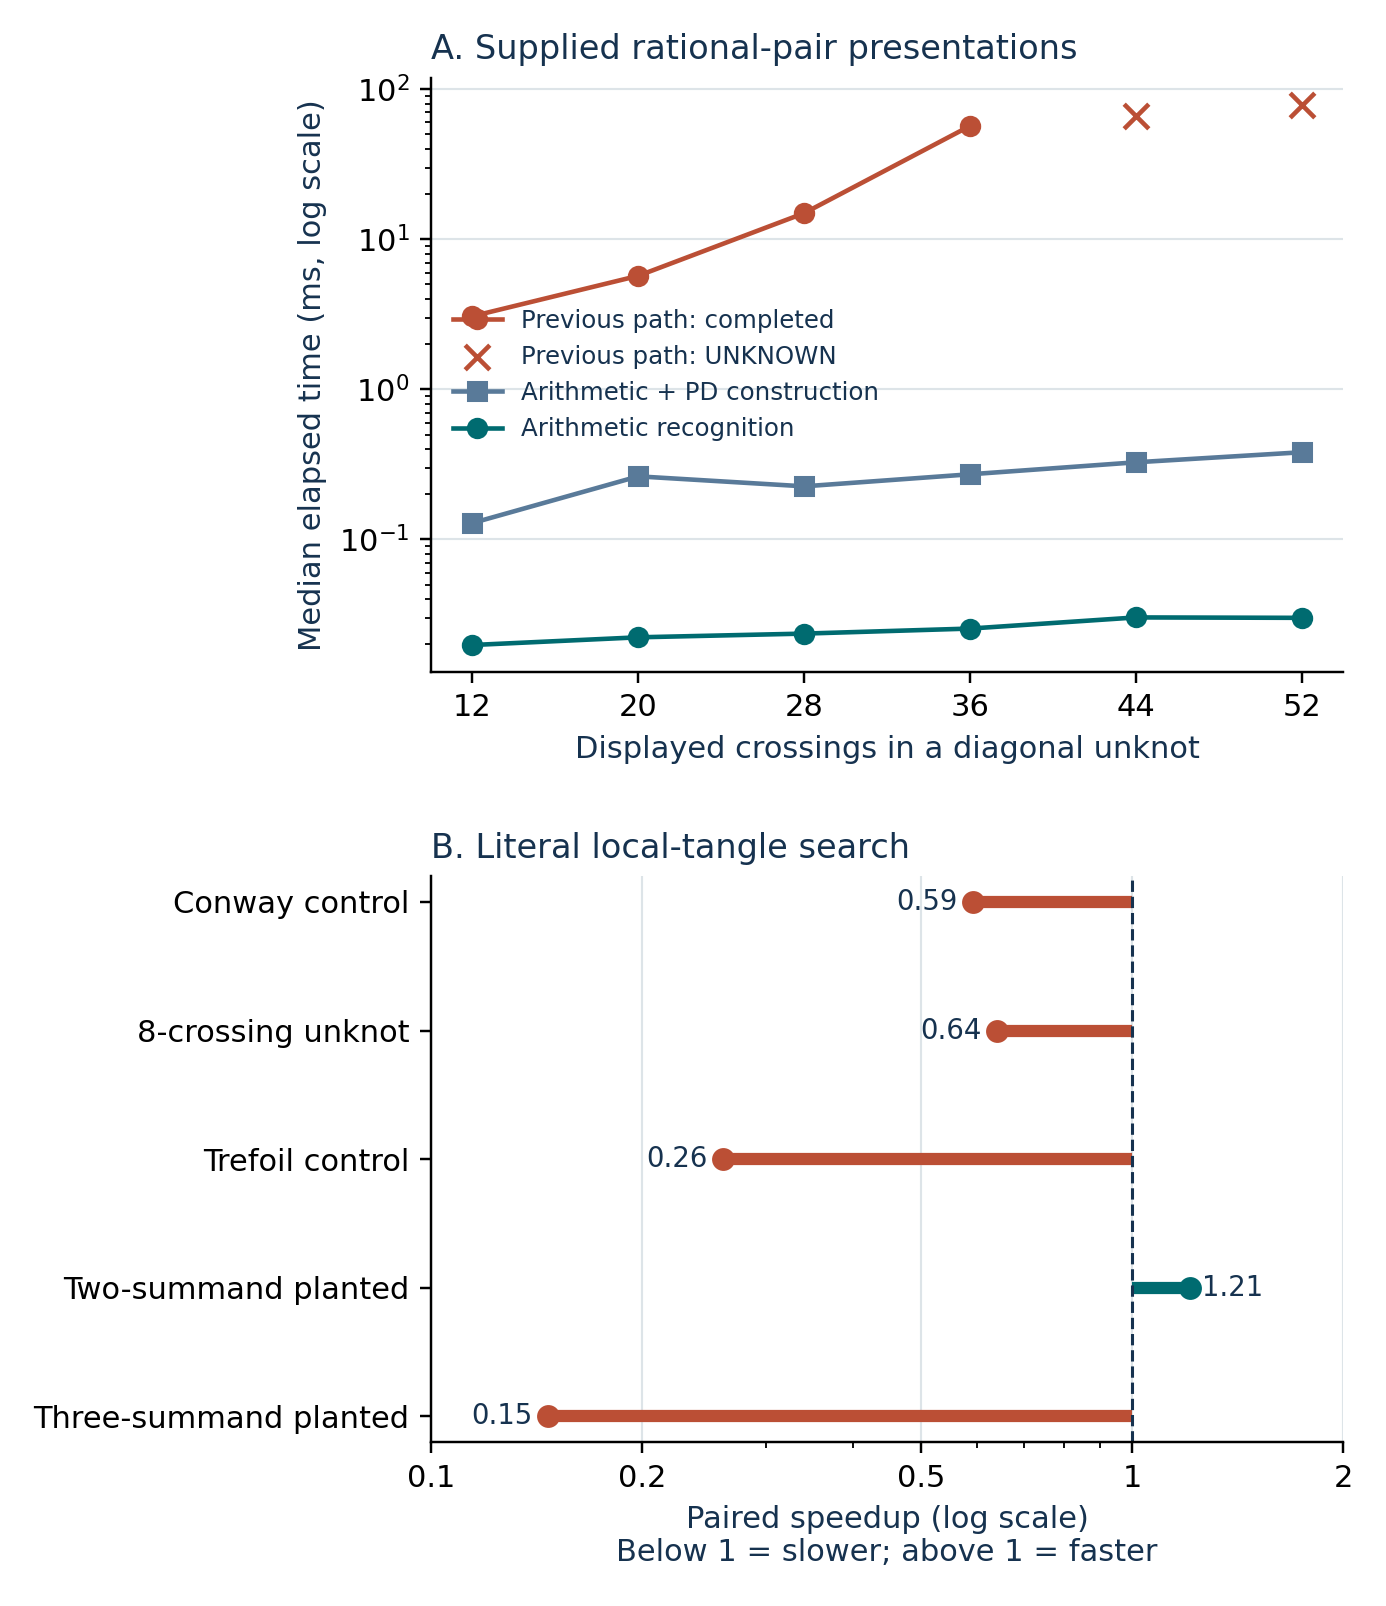
\includegraphics[width=\textwidth]{figures/benchmarks.png}
\caption{Recorded pipeline behavior. Top: diagonal unknot times, with
baseline cap exits marked separately from completed decisions. Bottom:
the optional local wrapper's paired speedups, including all measured
regressions. The figure is generated from the supplied JSON, not fitted
to an asymptotic model.}
\label{fig:benchmarks}
\end{figure}
}{}

\subsection{Reproducibility limits and useful follow-up measurements}

The archive's benchmark driver records every timing sample, both baseline
result objects and one new-path result per structured round. Local rounds
retain all three result objects. Recorded evidence includes methods, available
scan statistics, and the baseline before/after control ratio; end-to-end
and compressed calls retain their timing samples and stated summaries. It can regenerate the source examples and
planted PDs. The plotting script reads the recorded JSON and requires no
new timing run. A separate reproducibility driver exposes the quick tests,
full suite, mathematical diagnostics, and optional repeated benchmarks.

The measurements establish performance for these sources and this
environment. They do not establish average-case behavior on random knots,
the effectiveness of discovering hidden Montesinos structure, or the
maximum performance of every pre-existing backend. In particular, the
primary ablation compares the new arithmetic branch to the default
previous path, not to a competition among all backend settings.
The useful next comparisons are plain-PD rational extraction, pipeline
placement of local search, stronger adversarial source scrambling,
independent environments, and accounting for expanded diagram construction.
The mathematical quadratic arithmetic bound rests on the proof above,
not on fitting the six compressed timing points.

% ===== 07_research.tex =====
\section{A precise route toward quasi-polynomial complexity}
\label{sec:roadmap}

The new arithmetic stage is polynomial on its supplied input class.
The bounded-description search is quasi-polynomial on a restricted
one-sided discovery problem. Neither result bounds the cost of the
remaining general instances. The objective now is to identify an interface
and a discovery theorem that can survive those instances without
materializing the exponential objects isolated above.

\subsection{Which compression target should be changed}

There are at least four different mathematical contracts for a tangle
summary:
\begin{enumerate}
\item \emph{Relative-boundary isotopy information.}
A rational slope determines a rational tangle up to isotopy fixing its
marked boundary. This is exact topological information, compactly encoded.
\item \emph{Full homotopy information.}
A Bar--Natan complex retains enough data to compute the homology of every
planar composition. Explicit representatives can be exponentially large
at the prescribed checkpoints of Section~\ref{sec:unknot-checkpoint-lower-bound}.
\item \emph{All Boolean continuation answers.}
The relation \(P\sim P'\) means that every allowed continuation produces
the same unknot decision. Section~\ref{sec:rational-continuation-rank}
shows exponentially many classes even for a fixed four-point boundary.
It also rules out a small linear factorization of that final Boolean
predicate on the constructed family.
\item \emph{A certificate for the actual input.}
A Montesinos arithmetic proof or a forbidden local disk can decide
one input without constructing all continuation answers. This is the
contract used by the delivered early exits.
\end{enumerate}

These contracts should be reflected in types and function boundaries.
A local nontriviality witness cannot be inserted as a substitute for a
full chain complex at an arbitrary internal node. A rational slope can
represent the topology of a rational piece, but this alone does not provide
a fast operation for gluing it to an arbitrary nonrational complex.
The required operation must either have its own theorem or retain the
original diagram for an exact fallback.

The rank-two identity
\[
 D_m=ps^{\mathsf T}-qr^{\mathsf T},
 \qquad H_m=\mathbf1\{|D_m|=1\}
\]
illustrates a productive distinction. A low-dimensional arithmetic value
can encode an exact answer after a nonlinear readout even when the
Boolean connection matrix has full rank. State-count and Boolean-rank
obstructions should therefore be used to reject an unsuitable
representation contract, not to reject all arithmetic approaches.

\subsection{What the proved restricted discovery theorem actually buys}

Proposition~\ref{prop:mon:bounded-discovery} removes the need for a
supplied occurrence map on a specified family. It is a genuine algorithm:
enumerate bounded sources, reject arithmetic or component failures,
compile a literal plane pattern, and propagate each possible root image.
When \(h=O(\log n)\), its running time is \(n^{O(\log n)}\), including
bit arithmetic and the polynomial work per candidate.

The quantifiers are the important part. Completeness holds for forbidden
tangles that already appear as literal admissible diagrams with the
specified source bound, orientation, and four distinct external edges.
The algorithm does not search arbitrary isotopies. It does not prove
that every nontrivial diagram contains a short witness of this kind.
It also never certifies an unknot merely because no forbidden template
was found.

The hypothesis is substantial. A continued fraction with a long sequence
of coefficients equal to two can have \(h=\Theta(n)\); storing its slope
still takes only \(O(n)\) bits, but the enumeration theorem's logarithmic
coefficient-count hypothesis need not hold. Conversely, a large twist
coefficient can contribute many displayed crossings while occupying one
coefficient slot. This explains why coefficient count is useful and why
it is not a universal measure of diagram difficulty.

The fixed catalogue already gives a concrete scalable rejection family
with arbitrary exteriors: every accepted literal occurrence of
\(R(1/3)+R(1/4)\), for example, proves nontriviality regardless of the
number or complexity of exterior crossings. A useful next theorem would
enlarge this family through certified local rewrites or a rational-region
extractor while preserving a proved total discovery bound.

\subsection{A hierarchy accounting criterion}

The geometric hierarchy route is complementary to the arithmetic tangle
route. It should be audited using the iteration count and operation cost
as separate parameters.

\begin{proposition}[Conditional accounting, not a new hierarchy theorem]
\label{prop:hierarchy-accounting}
Suppose a fully specified implementation has at most \(L(g+1)^L\)
elementary hierarchy events, as in the iteration estimate of
\cite[Proposition~9.1]{lackenby-2026}. Suppose additionally that
\[
 g\le n^a,\qquad L\le b(\log(n+2))^c
\]
for fixed constants \(a,b,c>0\), and that all encoding growth and
bit operations at each event are bounded by
\(\exp(O((\log(n+2))^{c+1}))\).
Then its total bit time has the same form
\[
 \exp(O((\log(n+2))^{c+1})).
\]
In particular, \(c=1\) yields \(n^{O(\log n)}\), whereas \(c=2\)
yields \(n^{O((\log n)^2)}\).
\end{proposition}

\begin{proof}
Taking logarithms of the event bound gives
\[
 \log L+L\log(g+1)
 =O((\log(n+2))^{c+1}).
\]
Multiplying the number of events by the assumed per-event bound adds
two quantities of that order in the exponent. This accounts for both
iteration count and operation cost. It proves no one of the hypotheses.
\end{proof}

This accounting is useful precisely because each hypothesis can fail
independently. A short hierarchy does not ensure short coordinate
descriptions. A combinatorially decreasing potential does not bound the
cost of finding the next compression. Replacing a surface by a compressed
description does not make intersection and update operations efficient
without an explicit algorithm. These obligations are central to turning
the hierarchy programme into a reviewed implementation.

The present tangle lower bounds do not refute such a geometric approach.
They concern specific algebraic summaries. Their practical lesson is
that geometric events should not be forced through an explicit full
complex merely to preserve an interface whose information is richer
than the decision requires.

\section{Further research questions and concrete milestones}
\label{sec:questions}

The following questions are ordered roughly from immediately actionable
implementation work to broader mathematical objectives. Each specifies
what would count as progress. They are research proposals, not assumptions
used to justify the existing code.

\begin{researchquestion}[Certified extraction of visible rational regions]
Can a validated PD be reduced to maximal visible rational regions in
\(O(n\log n)\) or another explicit polynomial time, while returning
relative-boundary isotopy certificates and exact slopes?
\end{researchquestion}
Start with bigon chains and the inverse operations of the rational compiler,
retaining cyclic port order, crossing signs, and a replayable contraction
tree. A useful first result would recognize the supplied diagonal family
after source metadata is removed and after arbitrary relabeling and
crossing reordering. A stronger result would admit carefully specified
flypes or local isotopies. The theorem should define which diagrams
the extractor is complete on, and charge each graph update rather than
assuming repeated scans are free.

\begin{researchquestion}[Choosing the placement of local search]
Can local obstruction search run after all cheaper certificates and before
the expensive fallback with a small, provable overhead bound?
\end{researchquestion}
The current negative controls already demonstrate why this matters.
Measure construction, validation, compilation, discovery, and fallback
separately, using held-out hosts as well as planted patterns. Share target
dart arrays and precompiled templates. A useful release gate is an
end-to-end improvement on difficult plain PDs while bounding overhead on
trefoils, descending diagrams, and homogeneous examples. A benchmark
selected only from successful local witnesses would not answer the question.

\begin{researchquestion}[Practical bounded-description enumeration]
Can the \(n^{O(h)}\) enumeration be pruned substantially without losing
completeness for its stated literal class?
\end{researchquestion}
Possible exact pruning keys include expansion size, endpoint pairing,
crossing-sign counts, rooted ribbon neighborhoods, and arithmetic residues.
Canonicalization must respect the difference between two isotopic rational
sources and two different literal diagrams: equality of slopes is enough
for isotopy, but not necessarily enough for an unmodified dart match.
An implementation should return the same existence answer as the exhaustive
small-\(h\) reference enumerator before any asymptotic speed claim is made.

\begin{researchquestion}[A larger certified local-tangle language]
Which arborescent or graph-manifold tangle classes admit compact peripheral
data and complete tests for whether an unknotting complement can exist?
\end{researchquestion}
The Montesinos criterion uses more than homology order: its congruence
condition excludes \(R(1/3)+R(1/4)\) even though the numerator and denominator
determinants are coprime. An extension should retain the exact boundary
slopes, exceptional-fiber information, and marking needed for gluing.
It should classify rational and product degeneracies explicitly. Merely
recording the first homology group of each piece loses the peripheral
information that makes the current obstruction effective.

\begin{researchquestion}[Typed arithmetic composition with an arbitrary exterior]
What exact interface permits a rational slope or a compact Seifert piece
to interact with a nonrational remainder without expanding its full complex?
\end{researchquestion}
A first milestone could support one rational piece glued to a small explicit
remainder with a polynomial cost in its bit description and the remainder's
actual size. The correctness theorem must specify which topological or
homological answer the interface preserves. There should be explicit
conversion and fallback rules. A compact slope object is not automatically
an object of the pre-existing chain-complex category.

\begin{researchquestion}[Continuation-dependent processing of the Pell family]
Can a general PD strategy detect and exploit the relationship between
prefix and actual suffix before it reaches the exponential checkpoint?
\end{researchquestion}
On the diagonal family, the decisive relation is the unimodular pairing
\(p_ks_k-q_kr_k=-1\). An algorithm that deliberately constructs the
full prefix complex pays for information that the suffix immediately
collapses. A useful experiment would compare symmetric gluing,
look-ahead, and arithmetic extraction on source-erased diagrams with
controlled perturbations. A useful theorem would bound the size of all
intermediate representations for that algorithm, rather than only
bounding the final unknot rank.

\begin{researchquestion}[Compact homological data beyond multiplicities]
Can differentials and extension data for structured tangle complexes be
stored in an arithmetic circuit, recurrence, or other succinct form on
which the needed closure operations remain efficient?
\end{researchquestion}
The lower bound permits such representations because it counts expanded
summands. It does not prove they exist with efficient operations.
A scalar multiplicity alone omits differential data; capping a multiplicity
can be unsound if later maps interact with its copies. The target should
include composition, cancellation, restriction to a justified homological
window, and exact rank decisions on the permitted output, with explicit
bit-growth bounds. Symbolic expression size must be analyzed alongside
the number of graph nodes in the representation.

\begin{researchquestion}[Useful arithmetic values before a nonlinear readout]
Which intermediate arithmetic invariants have a low-dimensional gluing
law but a sufficiently strong exact terminal predicate?
\end{researchquestion}
The signed determinant pairing is a complete example on rational
continuations. It converts a rank-two arithmetic matrix into a full-rank
Boolean matrix by testing membership in \(\{1,-1\}\).
For more general pieces, one might study peripheral matrices, presentations
with controlled relations, or exact equations for distinguished fillings.
An arithmetic invariant that is not complete should remain a one-sided
filter. In particular, a compact Jones or Euler calculation should not be
promoted to a general unknot detector without an additional theorem.

\begin{researchquestion}[Generalized representation lower bounds]
Can the continuation construction distinguish other proposed summary
models, including bounded-degree nonlinear readouts, compressed modules,
or restricted arithmetic circuits?
\end{researchquestion}
Any proposed lower bound must specify the model and its input encoding.
The current identity matrix already implies that a representative-subfamily
scheme preserving the existence of an accepting prefix for every displayed
suffix must retain all \(2^m\) prefixes: suffix \(Q_w\) accepts only \(P_w\).
This does not prevent a symbolic set representation. A stronger useful
result would identify exactly which operations force expansion and which
ones preserve compactness, rather than claiming a general complexity
separation from a state count.

\begin{researchquestion}[Sharper, simpler independent verification]
Can the separate Montesinos verifier be reduced from the conservative
cubic bound to \(O(B^2)\), or better with fast arithmetic, without merely
reusing the production implementation?
\end{researchquestion}
The nested replay exists to check tracked prefix statistics, not to decide
the topology. One option is to remove nonessential statistics from the
mathematical certificate and verify them separately. Another is to maintain
independent prefix products or use a product tree. The important outcome is
an independent small checker with a transparent source-to-fraction and
fraction-to-verdict proof, not a second function that trusts the producer.

\begin{researchquestion}[Short positive certificates and formal proof kernels]
Can a determinant-one arithmetic decision be turned into a compact,
replayable topological certificate and formalized in the ProveIt setting?
\end{researchquestion}
For compressed sources, a fully expanded Reidemeister movie may be longer
than the source by an exponential factor. A suitable certificate should
instead record rational-tangle identities, Euclidean arithmetic, and
boundary-preserving gluing steps in compressed form. Its checker must
verify all signs and primitive pairs. For local negative certificates,
the disk lemma can be formalized as a statement about finite dart
permutations and a plane embedding, with the imported topological theorem
kept explicit. Formalizing the disjoint-cone and triangle-representation
lemmas would give smaller initial proof-assistant milestones.

\begin{researchquestion}[Extending the local certificate geometry]
Can the implementation safely admit two ports on a single exterior edge,
disconnected crossing shadows with simple arcs, or additional boundary
marking conventions?
\end{researchquestion}
The initial four-distinct-edge contract avoids these cases and is sound.
An extension needs a new explicit cut-point representation and a proof
that the accepted common face still bounds the intended disk with no
hidden components. Disconnected shadows require more than simply
reusing root propagation from one component. Separate topology lemmas
and adversarial tests should precede any expansion of the accepted class.

\begin{researchquestion}[A useful structural completeness theorem]
Can every diagram in a broad, explicitly specified class be transformed
or decomposed so that arithmetic classification or a short forbidden
local certificate becomes available within quasi-polynomial cost?
\end{researchquestion}
Candidate classes should be defined by their diagrams and allowed moves,
not retrospectively by whether the implementation succeeds.
One could begin with a controlled arborescent grammar or diagrams with
a supplied decomposition tree and then study discovery.
Both the transformation count and the size of each intermediate diagram
or compressed source must be bounded. The current results provide
neither a universal \(O(\log n)\) coefficient bound nor a theorem that
local forbidden tangles cover all nontrivial knots.

\begin{researchquestion}[Hierarchy operation costs and the logarithmic exponent]
Can the geometric hierarchy programme supply executable bounds for
compression discovery, parallelity-bundle updates, boundary-pattern
simplification, and terminal checks, with controlled coordinate growth?
\end{researchquestion}
The accounting in Proposition~\ref{prop:hierarchy-accounting} identifies
the necessary parameters. An implementation audit should attach an
explicit representation and cost to each operation from the mathematical
algorithm. It should separately establish whether the needed hierarchy
length is \(O(\log n)\) or \(O((\log n)^2)\), since those produce
different quasi-polynomial exponents under polynomial pattern complexity.
A declining hierarchy potential alone is insufficient.

\begin{researchquestion}[Adversarial families and fair backend comparisons]
Which examples remain hard after provenance is removed, cheap certificates
are applied, and the best supported existing backend is selected?
\end{researchquestion}
The current diagonal family isolates a real expanded-complex problem;
the Alexander-one family isolates the failure of a common invariant;
the planted local hosts test certificate discovery. A broader study should
separate these purposes and include source-erased rational diagrams,
hidden local patterns, examples with no matches, and alternate compositions.
Keep resource exits censored, use fresh caches, report process startup
when relevant, and compare end-to-end time as well as inner kernels.
This would guide algorithm design without confusing favourable source
metadata with a general discovery improvement.

\subsection{Recommended sequence of follow-up contributions}

The next contribution should implement and certify visible rational-region
extraction, then benchmark the present arithmetic decision on ordinary
source-erased PDs. That would remove the largest practical qualification
from the supplied-source speedups on an explicit class.

A second contribution should move or schedule local search using the
measured pipeline costs, add an exact small-\(h\) reference enumerator,
and develop completeness-preserving pruning. Its claim should remain a
local-witness discovery bound until a wider structural theorem is proved.

A third contribution should implement one typed arithmetic/exterior
composition operation with a full correctness proof and a proved bound on
all intermediate representations. The Pell checkpoint family gives a sharp
test: success should avoid the expanded \(p_k+q_k\) cost, not simply hide
it in a later conversion step.

The broad quasi-polynomial objective then requires a coverage or hierarchy
theorem together with executable operation costs. The delivered arithmetic
and local certificate stages are exact components available for that
programme. The lower bounds identify a representation choice that can
defeat the programme even on unknots, while the arithmetic construction
demonstrates a concrete way around it in a mathematically complete case.

% ===== 08_appendix_references.tex =====
\appendix
\section{Algorithm summaries and size accounting}
\label{sec:appendix}

The following pseudocode fixes the arithmetic decisions independently of
the language-specific implementation. Fractions remain primitive because
each recurrence is unimodular. The integer accumulator is deliberately
not reduced as a rational number.

\begin{lstlisting}
PrimitiveFraction([a0, ..., ak]):
    (p, q) := (1, 0)
    for a in [ak, ..., a0]:
        (p, q) := (a*p + q, p)
    reject unsupported final infinity if q = 0
    if q < 0: (p, q) := (-p, -q)
    return (p, q)

MontesinosDecision(e, source_blocks):
    exceptional := []
    for block in source_blocks:
        (p, q) := PrimitiveFraction(block)
        (a, beta) := EuclideanDivmod(p, q)
        e := e + a
        if q > 1:
            append (beta, q) to exceptional
    (D, Q) := (e, 1)
    for (beta, alpha) in exceptional:
        (D, Q) := (D*alpha + beta*Q, Q*alpha)
    reject input outside the knot domain if D is even
    if len(exceptional) >= 3:
        return KNOTTED, exceptional-fiber certificate
    if abs(D) = 1:
        return UNKNOT, two-bridge certificate
    return KNOTTED, determinant certificate
\end{lstlisting}

The local obstruction checker uses the unnormalized primitive slopes as
well:
\begin{lstlisting}
ForbiddenLocalSource(source):
    require integer term e = 0
    require at least two finite nonintegral rational summands
    compute primitive (pi, qi), with qi > 1
    require two open strands and no closed component
    if number_of_summands >= 3: return FORBIDDEN
    Q := q1*q2
    F := p1*q2 + p2*q1
    return (F mod Q) not in {1, Q - 1}

FindLiteralWitness(host, source):
    compile and verify connected plane pattern with four ports
    require ForbiddenLocalSource(source)
    for target_root in crossings(host):
        for offset in {0, 2}:
            propagate the unique possible map over internal edges
            reject collisions, inconsistent rotations, or overpair errors
            check every remaining dart and four distinct outgoing edges
            if all source and separating-disk checks pass:
                return source, crossing map, rotations
    return UNKNOWN
\end{lstlisting}

\begin{table}[htbp]
\centering\small
\begin{tabularx}{\textwidth}{L{0.30\textwidth}L{0.25\textwidth}X}
\toprule
Operation & Bound & Input and scope\\
\midrule
Two-twist rational summary and gluing &
\(O(m^2)\) bits of time &
Words of length \(m\); \(O(m)\) bits of arithmetic data\\
\addlinespace
Montesinos production arithmetic &
\(O(B^2)\) bits of time &
Complete compressed source length \(B\), including delimiters\\
\addlinespace
Independent branch verification &
\(O(B^3)\) bits of time &
Valid \(O(B)\)-size certificates; parse purported input as well\\
\addlinespace
Literal PD construction &
Polynomial in \(B+C\) &
Must charge \(C\) expanded crossings; cap checked before allocation\\
\addlinespace
One compiled pattern search &
\(O(nm)\) word operations &
Connected \(m\)-crossing pattern, indexed target already validated\\
\addlinespace
Public finite-catalogue wrapper &
\(O(n\log(n+2)+nM)\) word operations &
Total expanded pattern size \(M\), plus all source/compilation costs\\
\addlinespace
Bounded-description discovery &
\((n+2)^{O(h)}\) bit operations &
Literal admissible sources with at most \(h\) coefficients\\
\bottomrule
\end{tabularx}
\caption{Complexity statements and the input sizes they actually charge.
The abstract matching word bounds have indexed-array realizations.
The Python implementation's table operations use the usual table model.}
\label{tab:complexity}
\end{table}

For the expansion row, even a conservative implementation that revisits
the current explicit graph at each construction step performs polynomially
many operations in \(B+C\). The delivered compiler avoids unnecessary
whole-graph mirroring, but this report makes no finer worst-case compiler
claim than is needed. The production arithmetic bound applies before
any expansion and is the bound relevant to exponentially large twist
coefficients.

\section{Artifact map and reproducibility}

The main article driver is
\code{article/unknot_arithmetic_continuations.tex}. It is assembled from
numbered editable sections by \code{article/build_article.py}; all prose,
theorems, tables, and bibliography are included directly in the combined
driver. The optional plotted figure is used when its file exists, so
the standalone combined source can also compile without the figure assets.
The archive contains both the assets and a portable plotting script.

\begin{table}[htbp]
\centering\small
\begin{tabularx}{\textwidth}{L{0.41\textwidth}X}
\toprule
Path in the archive & Purpose\\
\midrule
\code{article/} & Combined and section TeX, PDF, build script,
supplementary BibTeX, and figure assets\\
\code{fast/} & Runnable updated recognizer, standard-library implementation,
tests, examples, certificates, and preserved license\\
\code{integration/} & Reviewable patch, application instructions, source
manifest, and patch byte-verification manifest\\
\code{experiments/} & Corpus generator, paired benchmark,
independent arithmetic and topology diagnostics, reproduction launcher\\
\code{examples/} & Complete structured and planted plain-PD inputs\\
\code{certificates/} & Complete local source-plus-map certificates\\
\code{results/} & Raw timings, finite verification outputs, full-suite
and patch-application logs\\
\code{RESEARCH_PROVENANCE.md} & Baseline, imported results,
independently derived claims, and limited inspiration attribution\\
\bottomrule
\end{tabularx}
\caption{Files supplied for review and later integration into ProveIt.}
\end{table}

The reproduction launcher accepts an explicit output directory and creates
an isolated replay workspace, leaving the bundled measurement record
unchanged. From any working directory, invoke its absolute path with
\code{--quick} for the added suites and finite diagnostics,
\code{--full-tests} for the full suite, \code{--identity} for all identity
matrices through \(m=10\), or \code{--benchmarks} for a fresh seven-round
timing run. The \code{--all} mode intentionally performs the expensive
reproductions as well. Exact examples are in the top-level README.

The repository patch was created for the pinned baseline, not for an
unseen future revision. Its manifest permits a reviewer to compare the
expected bytes before application. Subsequent repository changes may
require a normal patch merge and another targeted validation; that is
an integration issue rather than a change in any theorem above.

\begin{thebibliography}{99}
\small\raggedright

\bibitem{proveit-baseline}
V. Reshetnikov and contributors.
\emph{ProveIt: Topology/UnknotRecognition}.
Repository source and research reports, commit
\code{86f23490006c880cd01db9bec10761d39c6395c8},
inspected 8 October 2026.
\url{https://github.com/VladimirReshetnikov/ProveIt/tree/86f23490006c880cd01db9bec10761d39c6395c8/Topology/UnknotRecognition}.

\bibitem{kronheimer-mrowka}
P. B. Kronheimer and T. S. Mrowka.
\emph{Khovanov homology is an unknot-detector}.
arXiv:1005.4346, 2010.
\url{https://arxiv.org/abs/1005.4346}.

\bibitem{lackenby-2021}
M. Lackenby.
\emph{Unknot recognition in quasi-polynomial time}.
Oxford lecture slides, March 2021, especially slides 7 and 25--34.
The displayed announced bound is \(2^{O((\log n)^3)}\).
\url{https://people.maths.ox.ac.uk/lackenby/quasipolynomial-talk-oxford-compressed.pdf}.

\bibitem{lackenby-2026}
M. Lackenby.
\emph{Incompressible surfaces, hierarchies and unknot recognition}.
arXiv:2607.23350v1, 25 July 2026, especially Sections 9--10.
\url{https://arxiv.org/abs/2607.23350}.

\bibitem{kauffman-lambropoulou-tangles}
L. H. Kauffman and S. Lambropoulou.
On the classification of rational tangles.
\emph{Advances in Applied Mathematics} 33 (2004), 199--237.
arXiv:math/0311499.
\url{https://arxiv.org/abs/math/0311499}.

\bibitem{kauffman-lambropoulou-knots}
L. H. Kauffman and S. Lambropoulou.
On the classification of rational knots.
\emph{L'Enseignement Math\'ematique} 49 (2003), 357--410.
arXiv:math/0212011.
\url{https://arxiv.org/abs/math/0212011}.

\bibitem{KauffmanLambropoulouHard}
L. H. Kauffman and S. Lambropoulou.
\emph{Hard unknots and collapsing tangles}.
arXiv:math/0601525v5, 26 July 2014; original preprint 2006.
Especially Theorems 4--5 and the rational fraction conventions.
\url{https://arxiv.org/abs/math/0601525}.

\bibitem{KauffmanLambropoulouFractions}
L. H. Kauffman and S. Lambropoulou.
\emph{From tangle fractions to DNA}.
arXiv:math/0311511, 2003, especially Theorem 1 and Section 4.1.
\url{https://arxiv.org/abs/math/0311511}.

\bibitem{nogueira-salgueiro}
J. M. Nogueira and A. Salgueiro.
On embeddings of 2-string tangles into the unknot, the unlink and split links.
\emph{Topology and its Applications} 305 (2022), 107866.
arXiv:2110.15645v1, especially Proposition 4.4 and Theorem 4.9.
\url{https://arxiv.org/abs/2110.15645}.

\bibitem{belousov-pretzel}
Y. Belousov.
\emph{Explicit formulas for the Alexander polynomial of pretzel knots}.
arXiv:2502.10370v4, 9 March 2026.
\emph{Bulletin of the Australian Mathematical Society},
doi:10.1017/S0004972726101439.
Especially Theorem 1(3) and Section 2.3.
\url{https://arxiv.org/abs/2502.10370}.

\bibitem{BarNatanTangles}
D. Bar--Natan.
Khovanov's homology for tangles and cobordisms.
\emph{Geometry \& Topology} 9 (2005), 1443--1499.
arXiv:math/0410495, especially Theorem 2 and Section 7.
\url{https://arxiv.org/abs/math/0410495}.

\bibitem{KhovanovPatterns}
M. Khovanov.
Patterns in knot cohomology I.
\emph{Experimental Mathematics} 12 (2003), no.~3, 365--374.
arXiv:math/0201306, especially Section 3.
\url{https://arxiv.org/abs/math/0201306}.

\bibitem{ShumakovitchTorsion}
A. N. Shumakovitch.
Torsion of the Khovanov homology.
\emph{Fundamenta Mathematicae} 225 (2014), 343--364.
arXiv:math/0405474v2, 19 June 2018, Corollary 3.2.C.
\url{https://arxiv.org/abs/math/0405474}.

\bibitem{OpenAIMathContextSeparation}
OpenAI.
\emph{An exponential two-way deterministic state lower bound for one-way
liveness}, inspected source section on relation products and context
distinguishability. In the \code{openai/math} repository, commit
\code{adc7f1241b42e322a6451854ab7e4b4c146bf78a}, 2026.
Used only as inspiration for the standard context-separation argument;
no headline automata theorem is assumed here.
\url{https://github.com/openai/math/tree/adc7f1241b42e322a6451854ab7e4b4c146bf78a}.
The precise source path and blob hash are in the accompanying provenance.

\end{thebibliography}
\end{document}
